% Options for packages loaded elsewhere
\PassOptionsToPackage{unicode}{hyperref}
\PassOptionsToPackage{hyphens}{url}
%
\documentclass[
]{article}
\usepackage{lmodern}
\usepackage{amssymb,amsmath}
\usepackage{ifxetex,ifluatex}
\ifnum 0\ifxetex 1\fi\ifluatex 1\fi=0 % if pdftex
  \usepackage[T1]{fontenc}
  \usepackage[utf8]{inputenc}
  \usepackage{textcomp} % provide euro and other symbols
\else % if luatex or xetex
  \usepackage{unicode-math}
  \defaultfontfeatures{Scale=MatchLowercase}
  \defaultfontfeatures[\rmfamily]{Ligatures=TeX,Scale=1}
\fi
% Use upquote if available, for straight quotes in verbatim environments
\IfFileExists{upquote.sty}{\usepackage{upquote}}{}
\IfFileExists{microtype.sty}{% use microtype if available
  \usepackage[]{microtype}
  \UseMicrotypeSet[protrusion]{basicmath} % disable protrusion for tt fonts
}{}
\makeatletter
\@ifundefined{KOMAClassName}{% if non-KOMA class
  \IfFileExists{parskip.sty}{%
    \usepackage{parskip}
  }{% else
    \setlength{\parindent}{0pt}
    \setlength{\parskip}{6pt plus 2pt minus 1pt}}
}{% if KOMA class
  \KOMAoptions{parskip=half}}
\makeatother
\usepackage{xcolor}
\IfFileExists{xurl.sty}{\usepackage{xurl}}{} % add URL line breaks if available
\IfFileExists{bookmark.sty}{\usepackage{bookmark}}{\usepackage{hyperref}}
\hypersetup{
  pdftitle={R Module 1},
  pdfauthor={Alex Fout},
  hidelinks,
  pdfcreator={LaTeX via pandoc}}
\urlstyle{same} % disable monospaced font for URLs
\usepackage[margin=1in]{geometry}
\usepackage{color}
\usepackage{fancyvrb}
\newcommand{\VerbBar}{|}
\newcommand{\VERB}{\Verb[commandchars=\\\{\}]}
\DefineVerbatimEnvironment{Highlighting}{Verbatim}{commandchars=\\\{\}}
% Add ',fontsize=\small' for more characters per line
\usepackage{framed}
\definecolor{shadecolor}{RGB}{248,248,248}
\newenvironment{Shaded}{\begin{snugshade}}{\end{snugshade}}
\newcommand{\AlertTok}[1]{\textcolor[rgb]{0.94,0.16,0.16}{#1}}
\newcommand{\AnnotationTok}[1]{\textcolor[rgb]{0.56,0.35,0.01}{\textbf{\textit{#1}}}}
\newcommand{\AttributeTok}[1]{\textcolor[rgb]{0.77,0.63,0.00}{#1}}
\newcommand{\BaseNTok}[1]{\textcolor[rgb]{0.00,0.00,0.81}{#1}}
\newcommand{\BuiltInTok}[1]{#1}
\newcommand{\CharTok}[1]{\textcolor[rgb]{0.31,0.60,0.02}{#1}}
\newcommand{\CommentTok}[1]{\textcolor[rgb]{0.56,0.35,0.01}{\textit{#1}}}
\newcommand{\CommentVarTok}[1]{\textcolor[rgb]{0.56,0.35,0.01}{\textbf{\textit{#1}}}}
\newcommand{\ConstantTok}[1]{\textcolor[rgb]{0.00,0.00,0.00}{#1}}
\newcommand{\ControlFlowTok}[1]{\textcolor[rgb]{0.13,0.29,0.53}{\textbf{#1}}}
\newcommand{\DataTypeTok}[1]{\textcolor[rgb]{0.13,0.29,0.53}{#1}}
\newcommand{\DecValTok}[1]{\textcolor[rgb]{0.00,0.00,0.81}{#1}}
\newcommand{\DocumentationTok}[1]{\textcolor[rgb]{0.56,0.35,0.01}{\textbf{\textit{#1}}}}
\newcommand{\ErrorTok}[1]{\textcolor[rgb]{0.64,0.00,0.00}{\textbf{#1}}}
\newcommand{\ExtensionTok}[1]{#1}
\newcommand{\FloatTok}[1]{\textcolor[rgb]{0.00,0.00,0.81}{#1}}
\newcommand{\FunctionTok}[1]{\textcolor[rgb]{0.00,0.00,0.00}{#1}}
\newcommand{\ImportTok}[1]{#1}
\newcommand{\InformationTok}[1]{\textcolor[rgb]{0.56,0.35,0.01}{\textbf{\textit{#1}}}}
\newcommand{\KeywordTok}[1]{\textcolor[rgb]{0.13,0.29,0.53}{\textbf{#1}}}
\newcommand{\NormalTok}[1]{#1}
\newcommand{\OperatorTok}[1]{\textcolor[rgb]{0.81,0.36,0.00}{\textbf{#1}}}
\newcommand{\OtherTok}[1]{\textcolor[rgb]{0.56,0.35,0.01}{#1}}
\newcommand{\PreprocessorTok}[1]{\textcolor[rgb]{0.56,0.35,0.01}{\textit{#1}}}
\newcommand{\RegionMarkerTok}[1]{#1}
\newcommand{\SpecialCharTok}[1]{\textcolor[rgb]{0.00,0.00,0.00}{#1}}
\newcommand{\SpecialStringTok}[1]{\textcolor[rgb]{0.31,0.60,0.02}{#1}}
\newcommand{\StringTok}[1]{\textcolor[rgb]{0.31,0.60,0.02}{#1}}
\newcommand{\VariableTok}[1]{\textcolor[rgb]{0.00,0.00,0.00}{#1}}
\newcommand{\VerbatimStringTok}[1]{\textcolor[rgb]{0.31,0.60,0.02}{#1}}
\newcommand{\WarningTok}[1]{\textcolor[rgb]{0.56,0.35,0.01}{\textbf{\textit{#1}}}}
\usepackage{longtable,booktabs}
% Correct order of tables after \paragraph or \subparagraph
\usepackage{etoolbox}
\makeatletter
\patchcmd\longtable{\par}{\if@noskipsec\mbox{}\fi\par}{}{}
\makeatother
% Allow footnotes in longtable head/foot
\IfFileExists{footnotehyper.sty}{\usepackage{footnotehyper}}{\usepackage{footnote}}
\makesavenoteenv{longtable}
\usepackage{graphicx,grffile}
\makeatletter
\def\maxwidth{\ifdim\Gin@nat@width>\linewidth\linewidth\else\Gin@nat@width\fi}
\def\maxheight{\ifdim\Gin@nat@height>\textheight\textheight\else\Gin@nat@height\fi}
\makeatother
% Scale images if necessary, so that they will not overflow the page
% margins by default, and it is still possible to overwrite the defaults
% using explicit options in \includegraphics[width, height, ...]{}
\setkeys{Gin}{width=\maxwidth,height=\maxheight,keepaspectratio}
% Set default figure placement to htbp
\makeatletter
\def\fps@figure{htbp}
\makeatother
\setlength{\emergencystretch}{3em} % prevent overfull lines
\providecommand{\tightlist}{%
  \setlength{\itemsep}{0pt}\setlength{\parskip}{0pt}}
\setcounter{secnumdepth}{5}
\usepackage{booktabs}


\definecolor{output}{HTML}{fffbcf}


% add a background color to the verbatim environment
\let\oldv\verbatim
\let\oldendv\endverbatim

\def\verbatim{\par\setbox0\vbox\bgroup\oldv}
\def\endverbatim{\oldendv\egroup\fboxsep0pt \noindent\colorbox{output}{\usebox0}}
% png images should be 72x72 pixels

\usepackage{xcolor}
\usepackage{hyperref}
\hypersetup{
  colorlinks=true,
  linkcolor=blue!50!red,
  urlcolor=red!70!black
}
  

% define colors:
\definecolor{bonus}{HTML}{81c9a8}
\definecolor{reflect}{HTML}{ffdb80}
\definecolor{assessment}{HTML}{93b6ed}
\definecolor{progress}{HTML}{bba3cc}
\definecolor{video}{HTML}{d98780}
\definecolor{caution}{HTML}{ff6700}
\definecolor{feedback}{HTML}{cccccc}


% template block for all environments 
\newenvironment{specialblock}[3]
{
  \begin{center}
  \begin{tabular}
  {|>{\columncolor{#1}}p{0.9\textwidth}|}\hline\\
  \includegraphics[scale=0.1]{src/images/#2}
  \textbf{#3}
}
{\\\\\hline
  \end{tabular}
  \end{center}
}


% styling for all special blocks
\newenvironment{bonus}{
  \specialblock{bonus}{sun-fill.png}{Bonus}
}{\endspecialblock}

\newenvironment{reflect}{
  \specialblock{reflect}{lightbulb-fill.png}{Reflect}
}{\endspecialblock}

\newenvironment{assessment}{
  \specialblock{assessment}{pencil-fill.png}{Assessment}
}{\endspecialblock}

\newenvironment{progress}{
  \specialblock{progress}{pulse-line.png}{Progress Check}
}{\endspecialblock}

\newenvironment{video}{
  \specialblock{video}{vidicon-fill.png}{Video}
}{\endspecialblock}

\newenvironment{caution}{
  \specialblock{caution}{alarm-warning-fill.png}{Caution}
}{\endspecialblock}

\newenvironment{feedback}{
  \specialblock{feedback}{chat-1-fill.png}{Feedback}
}{\endspecialblock}
\usepackage{booktabs}
\usepackage{longtable}
\usepackage{array}
\usepackage{multirow}
\usepackage{wrapfig}
\usepackage{float}
\usepackage{colortbl}
\usepackage{pdflscape}
\usepackage{tabu}
\usepackage{threeparttable}
\usepackage{threeparttablex}
\usepackage[normalem]{ulem}
\usepackage{makecell}
\usepackage{xcolor}
\usepackage[]{natbib}
\bibliographystyle{apalike}

\title{R Module 1}
\author{Alex Fout\footnote{Department of Statistics, Colorado State University, \href{mailto:fout@colostate.edu}{\nolinkurl{fout@colostate.edu}}}}
\date{2020-07-08}

\begin{document}
\maketitle

{
\setcounter{tocdepth}{2}
\tableofcontents
}
\hypertarget{welcome}{%
\section{Welcome!}\label{welcome}}

Hi, and welcome to the R Module 1 (AKA STAT 158) course at Colorado State University!

This course is the first of three 1 credit courses intended to introduce the R programming language to those with little or no programming experience.

Through these Modules (courses), we'll explore how R can be used to do the following:

\begin{enumerate}
\def\labelenumi{\arabic{enumi}.}
\tightlist
\item
  Perform basic computations and logic, just like any other programming language
\item
  Load, clean, analyze, and visualise data
\item
  Run scripts
\item
  Create reproducible reports so you can explain your work in a narrative form
\end{enumerate}

In addition, you'll also be exposed to some aspects of the broader R community, including:

\begin{enumerate}
\def\labelenumi{\arabic{enumi}.}
\tightlist
\item
  R as free, open source software
\item
  The RStudio free software
\item
  Publicly available packages which extend the capability of R
\item
  Events and community groups which advocate for the use of R and the support of R users
\end{enumerate}

More detail will be provided in the Course Topics laid out in the next chapter.

\hypertarget{how-to-navigate-this-book}{%
\subsubsection{How To Navigate This Book}\label{how-to-navigate-this-book}}

To move quickly to different portions of the book, click on the appropriate chapter or section in the the table of contents on the left.
The buttons at the top of the page allow you to show/hide the table of contents, search the book, change font settings, download a pdf or ebook copy of this book, or get hints on various sections of the book.
The faint left and right arrows at the sides of each page (or bottom of the page if it's narrow enough) allow you to step to the next/previous section.
Here's what they look like:

\begin{figure}

{\centering 
\includegraphics{src/images/left_arrow} 
\includegraphics{src/images/right_arrow} 

}

\caption{Left and right navigation arrows}\label{fig:unnamed-chunk-1}
\end{figure}

\hypertarget{associated-csu-course}{%
\subsection{Associated CSU Course}\label{associated-csu-course}}

This bookdown book is intended to accompany the associated course at Colorado State University, but the curriculum is free for anyone to access and use.
If you're reading the PDF or EPUB version of this book, you can find the ``live'' version at \url{https://csu-r.github.io/Module1/}, and all of the source files for this book can be found at \url{https://github.com/CSU-R/Module1}.

If you're not taking the CSU course, you will periodically encounter instructions and references which are not relevant to you. For example, we will make reference to the Canvas website, which only CSU students enrolled in the course have access to.

\hypertarget{prelim}{%
\section{Course Preliminaries}\label{prelim}}

This course is presented as a \href{https://bookdown.org/}{bookdown} document, and is divided into chapters and sections
Each week, you'll be expected to read through the chapter and complete any associated exercises, quizzes, or assignments.

\hypertarget{special-boxes}{%
\subsubsection{Special Boxes}\label{special-boxes}}

Throughout the book, you'll encounter special boxes, each with a special meaning.
Here is an example of each type of box:

\begin{reflect}
This box will prompt you to pause and reflect on your experience and/or
learning. No feedback will be given, but this may be graded on
completion.
\end{reflect}

\begin{assessment}
This box will signify a quiz or assignment which you will turn in for
grading, on which the instructor will provide feedback.
\end{assessment}

\begin{progress}
This box is for checking your understanding, to make sure you are ready
for what follows.
\end{progress}

\begin{video}
This box is for displaying/linking to videos in order to help illustrate
or communicate concepts.
\end{video}

\begin{caution}
This box will warn you of possible problems or pitfalls you may
encounter!
\end{caution}

\begin{bonus}
This box is to provide material going beyond the main course content, or
material which will be revisited later in more depth.
\end{bonus}

\begin{feedback}
This box will prompt for your feedback on the organization of the
course, so we can improve the material for everyone!

Any of the boxes may include hyperlinks like this:
\href{https://www.r-graph-gallery.com/}{I am a link} or code like this
\texttt{This\ is\ code}.
\end{feedback}

\hypertarget{how-this-book-displays-code}{%
\subsubsection{How This Book Displays Code}\label{how-this-book-displays-code}}

In addition, you may see R code either as part of a sentence like this: \texttt{1+1}, or as a separate block like so:

\begin{Shaded}
\begin{Highlighting}[]
\DecValTok{1}\OperatorTok{+}\DecValTok{1}
\end{Highlighting}
\end{Shaded}

\begin{verbatim}
[1] 2
\end{verbatim}

Sometimes (as in this example) we will also show the \textbf{output} (in yellow), that is, the result of running the R code. In this case the code \texttt{1+1} produced the output \texttt{2}.
If you hover over a code block with your mouse, you will see the option to copy the code to your clipboard, like this:

\begin{figure}

{\centering 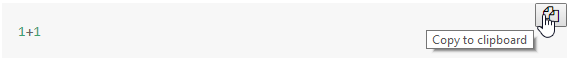
\includegraphics{src/images/copy_code} 

}

\caption{copying code from this book}\label{fig:unnamed-chunk-9}
\end{figure}

This will be useful when you are asked to run code on your computer.

\hypertarget{next-steps}{%
\subsubsection{Next Steps}\label{next-steps}}

When you're ready, go to the next section to learn about the course syllabus and grading policies.

\begin{feedback}
Any feedback for this section? Click
\href{https://docs.google.com/forms/d/e/1FAIpQLSePQZ3lIaCIPo9J2owXImHZ_9wBEgTo21A0s-A1ty28u4yfvw/viewform?entry.1684471501=Course\%20Preliminaries}{here}
\end{feedback}

\hypertarget{course-topics-syllabus}{%
\subsection{Course Topics \& Syllabus}\label{course-topics-syllabus}}

Broadly speaking, the topics of this course are described by the Chapter Titles. Here's what each entails:
- Course Preliminaries: Introduction to R and the world of R
- Installing R: Like it sounds, setting up your computer so you can work with R.
- R Programming Fundamentals: The basics of programming in R, the building blocks that you need in order to do anything more interesting.
- Working with Data: How to do meaningful things with data sets. Probably the most useful Chapter of the book.
- Creating R Programs: More programming concepts to increase your R Power!

\hypertarget{syllabus}{%
\subsubsection{Syllabus}\label{syllabus}}

First, some important details:

\begin{itemize}
\item
  \textbf{Instructor}: \href{mailto:fout@colostate.edu}{Alex Fout}
\item
  \textbf{Office Hours}: TBD on Microsoft Teams
\item
  \textbf{Webpages}: \href{https://canvas.colostate.edu}{Canvas}, \href{https://csu-r.github.io/Module1/}{this textbook}
\item
  \textbf{Course Credits}: 1. Because this week lasts four weeks, this course should ``feel'' like a 3 credit course for four weeks. Normally this means \textasciitilde3 hours of lecture and 12 hours of work outside of lecture per week. Because this course is online, there will be 1 hour or less of ``lecture'' (see below), and about 14 hours of outside work per week.
\item
  \textbf{Textbook}: You're reading it right now. The textbook will be your primary learning resource. You'll be expected to read through the required sections, watch any relevant videos, and complete any reflections, progress checks, and assessments along the way. On days when a quiz is due, you should complete the reading \emph{before} you take the quiz.
\item
  \textbf{Prerequisites}: None
\item
  \textbf{Progress Checks}: As you work your way through the textbook, you'll encounter purple ``Progress Check'' boxes. For Week 1, you'll submit your responses directly to canvas. For weeks 2-4, you'll fill in a R Markdown document and submit it to canvas. You'll be provided a template to fill in as you complete the progress checks. To turn in the document, you'll \textbf{knit} the document to HTML or PDF and upload to Canvas. (More details coming later in the book!). Progress checks will be graded on completion, organization, and correctness.
\item
  \textbf{Homework}: About once per week, you'll complete an assignment using R. Homeworks must be turned in by 11:59pm (Mountain) on the day they are due.
\item
  \textbf{Exams}: There will be no exams in this course
\item
  \textbf{Quizzes}: Once per week, there will be a 15 minute Canvas quiz. Quizzes must be completed by 11:59pm (Mountain) on the day they are due.
\item
  \textbf{Lectures}: Since we aren't having in-person lectures, we will hold short \emph{mini-lectures} instead (more details on Canvas). These will be shorter than a traditional lecture (approximately 10-30 minutes), and the purpose will be to allow some interaction between everyone in the course and to allow the instructor to introduce any relevant topics and address any challenges that students are having.
\item
  \textbf{Grading}: The grading for the course is apportioned like so:

  \begin{itemize}
  \tightlist
  \item
    Progress Checks: 30\%
  \item
    Homework: 40\%
  \item
    Quizzes: 30\%
  \end{itemize}
\end{itemize}

\hypertarget{schedule}{%
\subsubsection{Schedule}\label{schedule}}

\begin{table}[H]
\centering
\begin{tabular}{r|l|l|l|l}
\hline
Week & Weekday & Date & Reading & Due\\
\hline
1 & Monday & July 13 & Ch1, Ch2 & Progress Check 1\\
\hline
1 & Wednesday & July 15 & Ch3 & Quiz 1\\
\hline
1 & Friday & July 17 & Ch4 & Assignment 1\\
\hline
2 & Monday & July 20 & Ch4 & Progress Check 2\\
\hline
2 & Wednesday & July 22 & Ch4 & Quiz 1\\
\hline
2 & Friday & July 24 & Ch5 & Assignment 2\\
\hline
3 & Monday & July 27 & Ch5 & Progress Check 3\\
\hline
3 & Wednesday & July 29 & Ch5 & Quiz 1\\
\hline
3 & Friday & July 31 & Ch5 & Assignment 3\\
\hline
4 & Monday & August 03 & Ch6 & Progress Check 4\\
\hline
4 & Wednesday & August 05 & Ch6 & Quiz 4\\
\hline
4 & Friday & August 07 & Ch6 & Assignment 4\\
\hline
\end{tabular}
\end{table}

\hypertarget{course-policies}{%
\subsubsection{Course Policies}\label{course-policies}}

\begin{itemize}
\tightlist
\item
  \textbf{Late Work}: Homework and Progress Checks must be turned in on time to receive full credit. You may turn in Homework and Progress Checks up to 2 days late for up to 50\% credit.
\item
  \textbf{Group Work}: Students are welcome to discuss the course with each other, but all work you turn in must be your own. This means no sharing solutions to homework, progress checks, or quizzes. You may not work with other students on quizzes. You \emph{are} welcome to seek help on Canvas discussion boards and during office hours.
\item
  \textbf{Students with Disabilities}: The university is committed to providing support for students with disabilities. If you have an accommodation plan, please provide that to me as soon as possible so we can discuss appropriate arrangements.
\item
  \textbf{Growth Mindset}: This phrase was coined by Carol Dweck to reflect how your learning outcomes can be affected by the way you view the learning process. To quote Dweck: ``The view you adopt for yourself profoundly affects the way you lead your life\ldots{} Believing that your qualities are carved in stone - \emph{the fixed mindset} - creates an urgency to prove yourself over and over. If you have only a certain amount of intelligence, a certain personality, and a certain moral character --- well, then you'd better prove that you have a healthy dose of them. It simply wouldn't do to look or feel deficient in these most basic characteristics\ldots{} There's another mindset in which these traits are not simply a hand you're dealt and have to live with, always trying to convince yourself and others that you have a royal flush when you're secretly worried it's a pair of tens. In this mindset, the hand you're dealt is just the starting point for development. This growth mindset is based on the belief that your basic qualities are things you can cultivate through your efforts. Although people may differ in every which way --- in their initial talents and aptitudes, interests, or temperaments --- everyone can change and grow through application and experience.'' Programming may be a very new, intimidating thing for you. That's okay! View this course as a way to grow and gain new skills which you can use to do incredible and important things!
\item
  \textbf{Learn by doing}: \href{https://statistics.colostate.edu/person/?id=B0D2F899C79C05AAE4EDBA6EE2FECACA\&sq=t}{A wise statistics instructor} once compared watching someone else solve statistics problems to watching someone else practice shooting basketball free throws. You may learn a little by watching, but at some point you won't get any better until you try it yourself! The same can be said for programming. Reading a textbook and watching videos are a good \emph{start}, but you'll have to actually \emph{program} in order to get any better! This textbook was designed to be \emph{interactive}, and I encourage you to ``code along with the book'' as you read.
\end{itemize}

\hypertarget{grading-scale}{%
\subsubsection{Grading Scale}\label{grading-scale}}

Grades will be assigned according to the following scale:

\begin{table}[H]
\centering
\begin{tabular}{l|l}
\hline
Class\_Score & Letter\_Grade\\
\hline
92\%-100\% & A\\
\hline
90\%-92\% & A-\\
\hline
88\%-90\% & B+\\
\hline
82\%-88\% & B\\
\hline
80\%-82\% & B-\\
\hline
78\%-80\% & C+\\
\hline
70\%-78\% & C\\
\hline
60\%-70\% & D\\
\hline
0\%-60\% & F\\
\hline
\end{tabular}
\end{table}

\begin{feedback}
Any feedback for this section? Click
\href{https://docs.google.com/forms/d/e/1FAIpQLSePQZ3lIaCIPo9J2owXImHZ_9wBEgTo21A0s-A1ty28u4yfvw/viewform?entry.1684471501=Course\%20Topics\%20\%26\%20Syllabus}{here}
\end{feedback}

\hypertarget{running-your-first-r-code}{%
\subsection{Running your first R Code}\label{running-your-first-r-code}}

Enough of the boring stuff, let's run some R code!
Normally you will run R on your computer, but since you may not have R installed yet, let's run some R code using a website first.
As you run code, you'll see some of the things R can do.
In a browser, navigate to \href{https://rdrr.io/snippets/}{rdrr.io/snippets}, where you'll see a box that looks like this:

\begin{figure}

{\centering 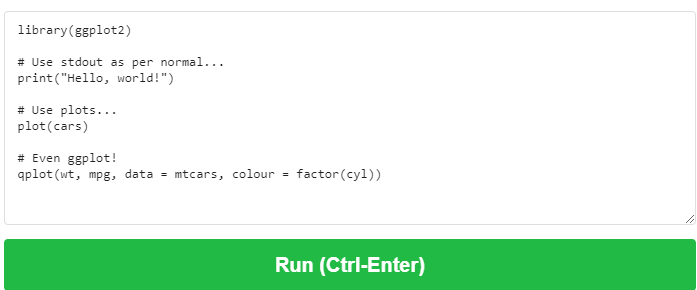
\includegraphics{src/images/rdrr} 

}

\caption{rdrr code entry box}\label{fig:unnamed-chunk-12}
\end{figure}

The box comes with some code entered already, but we want to use our own code instead, so delete all the text, from \texttt{library(ggplot2)} to \texttt{factor(cyl))}.
In its place, type \texttt{1+1}, then click the big green ``Run'' button.
You should see the \texttt{{[}1{]}\ 2} displayed below.
So if you give R a math expression, it will evaluate it and give the result.
Note: the ``correct answer'' to \(1+1\) is \texttt{2}, but the output also displays \texttt{{[}1{]}}, which we won't explain until later, so you can ignore that for now.

Next, delete the code you just wrote and type (or copy/paste) the following, and run it:

\begin{Shaded}
\begin{Highlighting}[]
\KeywordTok{factorial}\NormalTok{(}\DecValTok{10}\NormalTok{)}
\end{Highlighting}
\end{Shaded}

The result should be a very large number, which is equivalent to \(10!\), that is, \(10\times9\times8\times7\times6\times5\times4\times3\times2\times1\).
This is an example of an R \emph{function}, which we will discuss more later.

Aside from math, R can produce plots. Try copy/pasting the following code into the website:

\begin{Shaded}
\begin{Highlighting}[]
\NormalTok{x <-}\StringTok{ }\DecValTok{-10}\OperatorTok{:}\DecValTok{10}
\KeywordTok{plot}\NormalTok{(x, x}\OperatorTok{^}\DecValTok{2}\NormalTok{)}
\end{Highlighting}
\end{Shaded}

You should see points in a scatter plot which follow a parabola.
Here's a more complicated example, which you should copy/paste into the website and run:

\begin{Shaded}
\begin{Highlighting}[]
\KeywordTok{library}\NormalTok{(ggplot2)}
\KeywordTok{theme_set}\NormalTok{(}\KeywordTok{theme_bw}\NormalTok{())}
\KeywordTok{ggplot}\NormalTok{(mtcars, }\KeywordTok{aes}\NormalTok{(}\DataTypeTok{y=}\NormalTok{mpg, }\DataTypeTok{fill=}\KeywordTok{as.factor}\NormalTok{(cyl))) }\OperatorTok{+}\StringTok{ }
\StringTok{  }\KeywordTok{geom_boxplot}\NormalTok{() }\OperatorTok{+}\StringTok{ }
\StringTok{  }\KeywordTok{labs}\NormalTok{(}\DataTypeTok{title=}\StringTok{"Engine Fuel Efficiency vs. Number of Cylinders"}\NormalTok{, }\DataTypeTok{y=}\StringTok{"MPG"}\NormalTok{, }\DataTypeTok{fill=}\StringTok{"Cylinders"}\NormalTok{) }\OperatorTok{+}\StringTok{ }
\StringTok{  }\KeywordTok{theme}\NormalTok{(}\DataTypeTok{legend.position=}\StringTok{"bottom"}\NormalTok{, }
        \DataTypeTok{axis.ticks.x =} \KeywordTok{element_blank}\NormalTok{(),}
        \DataTypeTok{axis.text.x =} \KeywordTok{element_blank}\NormalTok{())}
\end{Highlighting}
\end{Shaded}

R can be used to make many types of visualizations, which you will do more of later.

\begin{bonus}
This may be the first time you've seen R, so it's okay if you don't
understand how to read this code. We'll talk more later about what each
statement is doing, but for now, here is a brief description of some of
the code above:

\begin{itemize}
\tightlist
\item
  \texttt{-10:10} This creates a sequence of numbers starting from -10
  and ending at 10. That is, \(-10, -9, -8, \ldots, 8, 9, 10\).
\item
  \texttt{library} This is a function which loads an R \emph{package}. R
  packages provide extra abilities to R.
\end{itemize}
\end{bonus}

\begin{feedback}
Any feedback for this section? Click
\href{https://docs.google.com/forms/d/e/1FAIpQLSePQZ3lIaCIPo9J2owXImHZ_9wBEgTo21A0s-A1ty28u4yfvw/viewform?entry.1684471501=Running\%20Your\%20First\%20R\%20Code}{here}
\end{feedback}

\hypertarget{getoutoftheclass}{%
\subsection{What do you hope to get out of this course?}\label{getoutoftheclass}}

To close out this chapter, it would be healthy for you to reflect on what you'd like to get from this course.
Take some time to think through each question below, and write down your answers.
It is fine if your honest answer is \emph{I don't know}.
In that case, try to come up with some possible answers that \emph{might} be true.

\begin{reflect}
\begin{enumerate}
\def\labelenumi{\arabic{enumi}.}
\tightlist
\item
  Why are you taking this course?
\item
  If this course is required for your major, how do you think it is
  supposed to benefit you in your studes?
\item
  What types of data sets related to your field of study may require
  data analysis?
\item
  What skills do you hope to develop in this course, and how might they
  be applied in your major and career?
\end{enumerate}
\end{reflect}

\begin{progress}
Submit your answers to the above reflection to Canvas.
\end{progress}

Store your answers in a safe place, and refer to them periodically as you progress through the course.
You may find that you aren't achieving your goals and that some adjustment to how you are approaching the course may be necessary.
Or you may find that your goals have changed, which is fine!
Just update your goals so that you have something to refer back to.

\begin{feedback}
Any feedback for this section? Click
\href{https://docs.google.com/forms/d/e/1FAIpQLSePQZ3lIaCIPo9J2owXImHZ_9wBEgTo21A0s-A1ty28u4yfvw/viewform?entry.1684471501=What\%20Do\%20You\%20Hope\%20To\%20Get\%20Out\%20Of\%20The\%20Class}{here}
\end{feedback}

\hypertarget{what-is-r}{%
\subsection{What is R?}\label{what-is-r}}

What is R? This question can be answered several different ways.
Here are a few of them:

\begin{feedback}
Any feedback for this section? Click
\href{https://docs.google.com/forms/d/e/1FAIpQLSePQZ3lIaCIPo9J2owXImHZ_9wBEgTo21A0s-A1ty28u4yfvw/viewform?entry.1684471501=What\%20is\%20R}{here}
\end{feedback}

\hypertarget{r-is-a-programming-language}{%
\subsubsection{R is a Programming Language}\label{r-is-a-programming-language}}

A programming language is a way of providing instructions to a computer.
Some popular languages (in no particular order) are C, C++, Java, Python, PHP, Visual Basic, and Swift.
Much like other types of languages, programming languages combine text and punctuation (syntax) to create statements which provide meaningful instructions (semantics) to be performed by a computer.
These instructions are called ``code''.
R code can be used to do many things, but primarily R was designed to easily work with data and produce graphics.
The R language can be used to use a computer to do the following:
- Read and process a set of data in a file or database
- Use data to compute statistics and perform statistical tests
- Produce nice looking visualizations of data
- Save data for others to use.
But this list is just the tip of the iceberg.
As you will see, R can be used to do so much more!
After the instructions are written, the R code is \emph{run}, that is, the code is provided to the computer, and the computer performs the instructions to produce the desired results.

\begin{bonus}
Many other programming languages use different syntax for the same
purpose.

\texttt{\#} comments out a line in R and python

\texttt{\%} comments out a line in matlab

\texttt{//} comments out a line in C++ and javascript

Similar to learning a foreign language, learning your first programming
language will make it easier to understand other similar ones.
\end{bonus}

\hypertarget{r-is-software}{%
\subsubsection{R is software}\label{r-is-software}}

R can also be thought of as the software program which runs R code.
In other words, if R code is the computer language, then the R software is what interprets the language and makes the computer follow the instructions laid out in the code.
This is sometimes called ``base R''.

\hypertarget{r-is-free}{%
\subsubsection{R is Free}\label{r-is-free}}

The R software is free, so anyone can download R, write R code, and run the R code in order to produce results on their computer.

\hypertarget{r-is-open-source}{%
\subsubsection{R is Open Source}\label{r-is-open-source}}

The R software, which runs R code, is also made up of a bunch of code called \emph{source code}.
In addition to being free, R is also \emph{open source}, meaning that anyone can look at the source code and understand the ``deep-down nuts-and-bolts'' of how R works.
In addition, anyone is able to \emph{contribute} to R, in order to improve it and add new features to it.

\begin{reflect}
What are the advantages of open-source software? What are some potential
downsides?

Why do you think the creators of R decided to make it open source?
\end{reflect}

\hypertarget{r-is-an-ecosystem}{%
\subsubsection{R is an ecosystem}\label{r-is-an-ecosystem}}

Another way of thinking about R is to include not only the R language and the R software, but also the community of R users and programmers, and the various ``add on'' software they have created for R.
These add on software are called ``packages''.

\hypertarget{r-packages}{%
\subsubsection{R Packages}\label{r-packages}}

An R package is software written to extend the capabilities of base R.
R packages are often written in R code, so anyone who knows how to write R code can also create R packages.
The importance of packages cannot be understated.
One of the reasons for the incredible popularity of R is the fact that members from the community can write new packages which enable R to do more.
Sometimes packages are written to help folks in particular disciplines (e.g.~psychology, geosciences, microbiology, education) do their jobs better.
Other times, packages are written to extend the capability of R so that people from many disciplines can use them.
R can be used to make web sites, interactive applications, dynamic reproducible reports, and even textbooks (like this one!).

The inclusion of R packages, combined with the free and open source nature of R software, has led to the development of a active, diverse, and supportive community of R users who can easily share their code, data, and results with one another.

\begin{bonus}
\href{https://github.com/ropensci/skimr}{skimr} provides a frictionless
approach to summary statistics which conforms to the principle of least
surprise, displaying summary statistics the user can skim quickly to
understand their data.
\end{bonus}

\hypertarget{r-interfaces}{%
\subsubsection{R Interfaces}\label{r-interfaces}}

The R software can be run in many different places, including personal computers, remote servers, and websites (as you have seen!).
R works on Windows, MAC OSX, and Linux, and
R can be run using a terminal or command line (if you know what those are), or using a graphical user interface (with buttons you can click and such).
By far one of the most popular ways of using R is with RStudio, which is \emph{also} open free and open source software.
For this course, you'll be using RStudio.

\begin{feedback}
Any feedback for this section? Click
\href{https://docs.google.com/forms/d/e/1FAIpQLSePQZ3lIaCIPo9J2owXImHZ_9wBEgTo21A0s-A1ty28u4yfvw/viewform?entry.1684471501=What\%20Is\%20R}{here}
\end{feedback}

\hypertarget{the-r-community}{%
\subsection{The R Community}\label{the-r-community}}

We already mentioned that there is active community of R users around the world, ranging from novice to expert level.
Here is a partial list of venues where R users interact (aside from the official websites, none of these links should be considered an official endorsement):

\begin{enumerate}
\def\labelenumi{\arabic{enumi}.}
\tightlist
\item
  \href{r-project.org}{R Project}: The official website for R
\item
  \href{https://www.r-project.org/mail.html}{R Project Mailing Lists}: Various email lists to stay informed on R related activities. The R-announce list is a good starting point, which will keep you updated on the latest releases of the R software
\item
  \href{https://twitter.com/hashtag/rstats?lang=en}{Twitter \#rstats}: Many R Users are active on Twitter and you can find them
\item
  \href{https://github.com/rfordatascience/tidytuesday}{Tidy Tuesday} is a weekly online project that focuses on understanding how to summarize, arrange, and make meaningful charts with open source data. You can see the projects others have done by following \#tidytuesday on twitter.
\item
  \href{https://rladies.org/}{R-Ladies} is a global group dedicated to promoting gender equality in the R community. They have an elaborate list of resources for learning and host educational and networking events.
\item
  \href{https://r-podcast.org/}{R-Podcast}: A periodic podcast with practical advice for using R, and the latest R news.
\item
  \href{r-bloggers.com}{R-Bloggers}: A blog website where authors can post examples of code, data analysis, and visualization.
\end{enumerate}

\hypertarget{places-to-get-help-if-youre-a-student-taking-this-class-for-credit}{%
\subsubsection{Places to Get Help (If you're a student taking this class for credit)}\label{places-to-get-help-if-youre-a-student-taking-this-class-for-credit}}

Students taking the course for credit should seek help from these places, in order:

\begin{itemize}
\tightlist
\item
  Canvas Discussion boards
\item
  Office Hours
\end{itemize}

I will not answer homework/quiz/textbook related questions via email

\hypertarget{places-to-get-help-anyone}{%
\subsubsection{Places to Get Help (anyone)}\label{places-to-get-help-anyone}}

If you find yourself stuck, there are many options available to you, here are a few:

\begin{enumerate}
\def\labelenumi{\arabic{enumi}.}
\tightlist
\item
  \href{https://stackoverflow.com}{Stack Overflow} is a message board where users can post questions about issues they're having. If you search for your error, there's likely already an answered question about it. If not, you can submit one with a \href{https://stackoverflow.com/questions/5963269/how-to-make-a-great-r-reproducible-example}{reproducible example} that the active community can help you with.
\item
  \href{https://cran.r-project.org/manuals.html}{R Manuals}: With so many R resources available on the internet, sometimes information get's ``boiled down'' or simplified for ease of communication. If you need the ``official answer'' to a question, these manuals are the place to go. Check out ``An Introduction to R'' for a good reference.
\end{enumerate}

\begin{feedback}
Any feedback for this section? Click
\href{https://docs.google.com/forms/d/e/1FAIpQLSePQZ3lIaCIPo9J2owXImHZ_9wBEgTo21A0s-A1ty28u4yfvw/viewform?entry.1684471501=The\%20R\%20Community}{here}
\end{feedback}

\hypertarget{installing-r}{%
\section{Installing R}\label{installing-r}}

In the previous chapter, you ran R code on a website.
The purpose of this chapter is to install R on your own computer, so that you can run R without needing access to the internet.

\begin{feedback}
Any feedback for this section? Click
\href{https://docs.google.com/forms/d/e/1FAIpQLSePQZ3lIaCIPo9J2owXImHZ_9wBEgTo21A0s-A1ty28u4yfvw/viewform?entry.1684471501=Installing\%20R}{here}
\end{feedback}

\hypertarget{computer-basics}{%
\subsection{Computer Basics}\label{computer-basics}}

If you're new to computers, this section will be important for you to get set up.
We'll briefly introduce some computer concepts and discuss how they're relevant to R.
If you understand the basics of operating systems, directory structures on your computer, and downloading/installing files, then you can probably skim this section, but be sure to pay attention to the R-specific information.

\hypertarget{operating-systems}{%
\subsubsection{Operating Systems}\label{operating-systems}}

An operating system is a set of programs that allow you to interact with the computer, and the most popular operating systems are Windows, Mac OS X, and Linux.
R works on Windows, Mac OS X, and several Linux-based operating systems, so if you have one of these operating systems, you'll be able install and use R.
At least, this is mostly true:

\begin{caution}
Some versions of Windows that run on ARM processors cannot install R,
and installing R on a Chromebook will likely be more complicated (see
\href{https://francish.netlify.app/post/installing-r-and-rstudio-on-a-pixel-slate/}{here}).
If you're in this situation, contact the instructor immediately.
\end{caution}

R isn't designed to work on tablets or phones which run mobile/tablet operating systems (like iOS, iPadOS, Android, ChromeOS), so these are not an option for R.

\hypertarget{files-directory-structures}{%
\subsubsection{Files \& Directory Structures}\label{files-directory-structures}}

A file is a collection of data stored on your computer's hard drive.
Examples of files include:

\begin{itemize}
\tightlist
\item
  A music file
\item
  A video
\item
  A slide presentation
\item
  A text document
\end{itemize}

Different types of files are often treated differently by your computer.
For example, a music file is played with a music player program, a video can be viewed with a video player, and a slide presentation might be viewed with Powerpoint.
Most operating systems know the type of a file by looking at the \emph{extension}, which is at the very end of the file's name.
Examples include ``.mp3'', ``.doc'', ``.txt'', and ``.ppt''.
When using R, we can write scripts which contain R code, and \emph{RMarkdown} documents, which include human readable text and code.
R scripts usually have either a ``.R'' or ``.r'' extension, and we'll also be using \emph{RMarkdown}, which use either a ``.Rmd'' or ``.rmd'' extension.

A \emph{directory}, or \emph{folder}, is a collection of files, and computers use directories to logically organize sets of files.
When working with R, you may have to organize several different types of files, including R code, data files, and images.
It will be important to stay organized when using R, and we will address this more later in the chapter.

With the increasing prevalence of the internet in everyday life, it's becoming less common for files to exist on your computer.
When writing R code, you'll be working with files on your computer, not accessing them over the internet.

\hypertarget{downloads-and-installations}{%
\subsubsection{Downloads and Installations}\label{downloads-and-installations}}

To install R, you'll have to download a file from the internet which performs the installation.
After you install R, you shouldn't have to download anything to run R.
The specific steps to install R will be different depending on your operating system, and this will be addressed in the next section.

\begin{feedback}
Any feedback for this section? Click
\href{https://docs.google.com/forms/d/e/1FAIpQLSePQZ3lIaCIPo9J2owXImHZ_9wBEgTo21A0s-A1ty28u4yfvw/viewform?entry.1684471501=Computer\%20Basics}{here}
\end{feedback}

\hypertarget{install-r-r-studio}{%
\subsection{Install R \& R Studio}\label{install-r-r-studio}}

Here's where you install R on your personal computer, but you'll actually be installing \emph{two} separate programs.
The \emph{first} is the R programming language.
The \emph{second} is a separate program called R Studio, which will be the primary way in which you interact with R in this class, we will say more about this later.

\hypertarget{installing-r-1}{%
\subsubsection{Installing R}\label{installing-r-1}}

Installation will look slightly different depending on the operating system, but the major steps are the same.

\begin{itemize}
\tightlist
\item
  First, navigate to the \href{https://cran.r-project.org/mirrors.html}{CRAN Mirrors Site}, which lists several locations from which R can be downloaded.
\item
  Find a location near you (or not, this isn't critical) and click on the link to be brought to the mirror site.
\end{itemize}

From this point, this will change depending on your operating system.

\hypertarget{windows}{%
\paragraph{Windows}\label{windows}}

\begin{itemize}
\tightlist
\item
  Click ``Download R for Windows'', then click ``base''.
\item
  Finally, Click ``Download R X.Y.Z for Windows'', where X, Y, and Z will be numbers. These numbers indicate which version of R you'll be installing. As of the publishing of this book, R is on version \texttt{r\_version}.
\item
  Your computer might prompt for the location on your computer that you would like to save the file. Select a location (reasonable options are your \texttt{Downloads} folder or the \texttt{Desktop}) and select ``save''.
\item
  When the download completes, find the downloaded file in the File Explorer and double click to run it. This will start the installation process.
\item
  Follow the on screen prompts. For the most part you can click ``next'' and ``install'' as appropriate, and you don't have to worry about changing any installation settings.
\item
  Click ``Finish'' to complete the installation!
\end{itemize}

\begin{video}
\href{https://youtu.be/7ZYn6q_pboE}{This video} shows the installation
process for Windows
\end{video}

\hypertarget{mac-os-x}{%
\paragraph{Mac OS X}\label{mac-os-x}}

\begin{itemize}
\tightlist
\item
  Click ``Download R for (Mac) OS X''
\item
  Click ``R-X.Y.Z.pkg'', where X, Y, and Z will be numbers. These numbers indicate which version of R you'll be installing. As of the publishing of this book, R is on version \texttt{r\_version}.
\item
  Your computer might prompt for the location on your computer that you would like to save the file. Select a location and select ``save''.
\item
  When the download completes, find the downloaded file in the Finder and double click to run it. This will start the installation process.
\item
  Follow the on screen prompts. For the most part you can click ``continue'', ``agree'', ``install'', as appropriate, and you don't have to worry about changing any installation settings.
\item
  Click ``Close'' to complete the installation!
\end{itemize}

\hypertarget{linux}{%
\paragraph{Linux}\label{linux}}

We will not provide details on installing R for Linux, because the process varies depending on your distribution, and because if you're using Linux, chances are you're more computer proficient than the average user.
Suffice it to say, The first step is:

\begin{itemize}
\tightlist
\item
  Click ``Download R for Linux''
\end{itemize}

And you can probably figure things out from there.

\hypertarget{conclusion}{%
\paragraph{Conclusion}\label{conclusion}}

You should now have R installed!
Technically speaking, nothing further is required to work with R.
You can open the RGui, and start coding immediately.
However, for this course we will be using RStudio, which is a very popular program with an incredibly rich set of features, which will enhance your R programming experience.

\hypertarget{installing-rstudio}{%
\subsubsection{Installing RStudio}\label{installing-rstudio}}

\begin{itemize}
\tightlist
\item
  Navigate to the \href{https://rstudio.com/products/rstudio/download/\#download}{RStudio Download Page}, and find the download file that matches your operating system.
\item
  Click the link to download the installer, which starts with ``RStudio-'' or ``rstudio-''.
\item
  Your computer might prompt for the location on your computer that you would like to save the file. Select a location (reasonable options are your \texttt{Downloads} folder or the \texttt{Desktop}) and select ``save''.
\item
  When the download completes, find the downloaded file and double click to run it. This will start the installation process.
\end{itemize}

From this point, this will change depending on your operating system.

\hypertarget{windows-1}{%
\paragraph{Windows}\label{windows-1}}

\begin{itemize}
\tightlist
\item
  Follow the on screen prompts. For the most part you can click ``next'' and ``install'' as appropriate, and you don't have to worry about changing any installation settings.
\item
  You should now be able to open the start menu, open the RStudio folder, and click on the RStudio icon to open RStudio
\end{itemize}

\begin{video}
\href{https://youtu.be/XnqENdiEb3I}{This video} shows the installation
process for Windows
\end{video}

\hypertarget{mac-os-x-1}{%
\paragraph{Mac OS X}\label{mac-os-x-1}}

\begin{itemize}
\tightlist
\item
  In the window which opens, drag the RStudio icon into the ``Applications'' folder. You may need to enter your password (click the ``Authenticate'' button) in order to do so.
\item
  You should now be able to navigate to the Applications folder in Finder, and click on the RStudio icon to open RStudio.
\end{itemize}

\hypertarget{conclusion-1}{%
\paragraph{Conclusion}\label{conclusion-1}}

\begin{bonus}
Rstudio also offers a \href{https://rstudio.cloud/}{cloud service} that
allows you to work with R in your browser. We'll use the desktop version
but you can check out the
\href{https://rstudio.cloud/learn/primers}{interactive primers} on the
cloud site.
\end{bonus}

\begin{feedback}
Any feedback for this section? Click
\href{https://docs.google.com/forms/d/e/1FAIpQLSePQZ3lIaCIPo9J2owXImHZ_9wBEgTo21A0s-A1ty28u4yfvw/viewform?entry.1684471501=Install\%20R\%20\%26\%20RStudio}{here}
\end{feedback}

\hypertarget{successfull-installation}{%
\subsection{Successfull Installation}\label{successfull-installation}}

When you successfully install R and RStudio, you should now be able to program in R!
Before moving further, you should become acquainted with the different parts of RStudio.
To do so, watch the video below:

\begin{video}
\href{https://youtu.be/w_3xp_3Sz6s}{This video} gives an introduction to
some of the main pieces of RStudio
\end{video}

\begin{feedback}
Any feedback for this section? Click
\href{https://docs.google.com/forms/d/e/1FAIpQLSePQZ3lIaCIPo9J2owXImHZ_9wBEgTo21A0s-A1ty28u4yfvw/viewform?entry.1684471501=Successfull\%20Installation}{here}
\end{feedback}

\hypertarget{running-code-in-rstudio}{%
\subsection{Running Code in RStudio}\label{running-code-in-rstudio}}

Now that you're somewhat familiar with RStudio, let's run the same code as we ran on the website, but this time let's run it in R.

\hypertarget{the-r-console}{%
\subsubsection{The R Console:}\label{the-r-console}}

In the \emph{R console}, type \texttt{1+1} and press enter.
The output in the console should look like the following:

\begin{figure}

{\centering 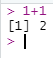
\includegraphics{src/images/1_plus_1_console} 

}

\caption{code in the console}\label{fig:unnamed-chunk-36}
\end{figure}

Notice that the output \texttt{2} is displayed, and the cursor is on a blank line, waiting for more input. This is how coding in the console works.

\hypertarget{r-scripts}{%
\subsubsection{R scripts}\label{r-scripts}}

Now let's run the same code, but in an R script.
If you haven't already, create a new R script by clicking on the \texttt{New\ File} icon, then selecting \texttt{R\ Script} like so:

\begin{figure}

{\centering 
\includegraphics{src/images/rstudio_newfile} 

}

\caption{code in the console}\label{fig:unnamed-chunk-37}
\end{figure}

In the script window which opens, type \texttt{1+1} and press enter.
Notice how now, the code did \emph{not} run?
In a script, you are free to write R code on several lines before you run it.
You can even save the script and load it later in order to run the code it contains.
There are multiple ways to run R code in a script.
To run a single line of code, do one of the following:

\begin{itemize}
\tightlist
\item
  Place the cursor on the desired line, hold the key, and press enter. On Mac OS X, hold key and press enter instead
\item
  Place the curse on the desired line and click the \texttt{Run} button that looks like this:
\end{itemize}

\begin{figure}

{\centering 
\includegraphics{src/images/rstudio_run} 

}

\caption{code in the console}\label{fig:unnamed-chunk-38}
\end{figure}

To run multiple lines of code, do one of the following:
- Highlight all the code you'd like to run, hold the key, and press enter. On Mac OS X, hold the key and press enter instead.
- Highlight all the code you'd like to run, and click the \texttt{Run} button.

Run the \texttt{1+1} code using one of the methods above, and observe the output.
Notice how the output is \emph{still} in the console window, even you ran the code in a script!

\begin{caution}
Even though running R code from the console and an R script are done
differently, they should produce the same results. Both are running R!
\end{caution}

Now that you've run some code in the console and from an R script, let's try some of the other code we wrote previously.

\hypertarget{same-examples-on-your-computer}{%
\subsubsection{Same Examples, On Your Computer!}\label{same-examples-on-your-computer}}

In the \emph{console}, type the command \texttt{factorial(10)}.
Did you get the same result as you got on the website?
Now type the following two lines in an R script and run them:

\begin{Shaded}
\begin{Highlighting}[]
\NormalTok{x <-}\StringTok{ }\DecValTok{-10}\OperatorTok{:}\DecValTok{10}
\KeywordTok{plot}\NormalTok{(x, x}\OperatorTok{^}\DecValTok{2}\NormalTok{)}
\end{Highlighting}
\end{Shaded}

This code produces a plot, which should show up in the lower right corner in the ``Plots'' window.
Finally, \emph{copy} the following code, paste it into your script, and run it:

\begin{Shaded}
\begin{Highlighting}[]
\KeywordTok{library}\NormalTok{(ggplot2)}
\KeywordTok{theme_set}\NormalTok{(}\KeywordTok{theme_bw}\NormalTok{())}
\KeywordTok{ggplot}\NormalTok{(mtcars, }\KeywordTok{aes}\NormalTok{(}\DataTypeTok{y=}\NormalTok{mpg, }\DataTypeTok{fill=}\KeywordTok{as.factor}\NormalTok{(cyl))) }\OperatorTok{+}\StringTok{ }
\StringTok{  }\KeywordTok{geom_boxplot}\NormalTok{() }\OperatorTok{+}\StringTok{ }
\StringTok{  }\KeywordTok{labs}\NormalTok{(}\DataTypeTok{title=}\StringTok{"Engine Fuel Efficiency vs. Number of Cylinders"}\NormalTok{, }\DataTypeTok{y=}\StringTok{"MPG"}\NormalTok{, }\DataTypeTok{fill=}\StringTok{"Cylinders"}\NormalTok{) }\OperatorTok{+}\StringTok{ }
\StringTok{  }\KeywordTok{theme}\NormalTok{(}\DataTypeTok{legend.position=}\StringTok{"bottom"}\NormalTok{, }
        \DataTypeTok{axis.ticks.x =} \KeywordTok{element_blank}\NormalTok{(),}
        \DataTypeTok{axis.text.x =} \KeywordTok{element_blank}\NormalTok{())}
\end{Highlighting}
\end{Shaded}

You're now running R code on your computer!

\begin{reflect}
Imagine you are practicing programming in R and your classmate tells you
they heard about an interesting new R command which they'd like you to
try out. Would you run the command in an R script, or the R console? How
might your answer change if you wanted to keep a record of all the
interesting R command you found?
\end{reflect}

\hypertarget{r-markdown}{%
\subsubsection{R Markdown}\label{r-markdown}}

You've seen how to run R code in the R console, and from an R script, but there's one more way to run R that we need to talk about: R Markdown

R scripts are convenient because they can store multiple R commands in one file.
R Markdown takes this idea further and stores code alongside human readable text.
There is much that could be said about R Markdown, but for now, we'll just stick with the basics.

To start, watch this video:

\begin{video}
\href{https://youtu.be/MhvipLohEfU}{This Video} gives a basic
introduction to RMarkdown.
\end{video}

As the video stated, there are three types of sections to an RMarkdown document:
- Header
- Human readable text
- Code Chunks

There's only one header, but there can be many blocks of human readable text and many code chunks.

\begin{bonus}
See
\href{https://rstudio.com/wp-content/uploads/2015/02/rmarkdown-cheatsheet.pdf}{here}
for more things you can do with RMarkdown.
\end{bonus}

\begin{caution}
As part of this class, you'll be filling in an R Markdown document as
you complete the progress checks in the book (except for the first
progress check box, which you completed already) On Canvas, download the
\texttt{progress\_check\_2.rmd} file and follow the instructions. Here
is the first code chunk you will include in the document!
\end{caution}

\begin{video}
TODO: Add video link. \href{}{This video} should help get you started
with the Progress Check Assignments!
\end{video}

\begin{feedback}
Any feedback for this section? Click
\href{https://docs.google.com/forms/d/e/1FAIpQLSePQZ3lIaCIPo9J2owXImHZ_9wBEgTo21A0s-A1ty28u4yfvw/viewform?entry.1684471501=Running\%20Code\%20in\%20RStudio}{here}
\end{feedback}

\hypertarget{workspace-setup}{%
\subsection{Workspace setup}\label{workspace-setup}}

Whenever you are programming in R, and especially for this class, it's important to stay organized.
This section will give you some instructions and tips for how to organize material for this R course

\hypertarget{recommended-settings}{%
\subsubsection{Recommended Settings}\label{recommended-settings}}

First of all, let's set some settings in RStudio.
At the top of the R window, click \texttt{Tools}, then \texttt{Global\ Options}, and do the following:

\begin{enumerate}
\def\labelenumi{\arabic{enumi}.}
\tightlist
\item
  On the left side of the window that pops up, and make sure it's on the ``General'' tab
\item
  Find the ``Workspace'' section on the right, make the following changes:
  -- \emph{uncheck} ``Restore .RData into workspace on startup''
  -- Change the ``Save workspace to .RData on exit'' option to \emph{never}
\item
  On the left side, select the ``Appearance'' tab.
\item
  (Optional) Change the Zoom setting to increase or decrease the size, to fit your screen best.
\item
  (Optional) Change the ``Editor theme:'' setting to find a color scheme that looks good to you.
\item
  Click ``Apply'', then ``OK'' at the bottom of the window.
\end{enumerate}

Step 2 ensures that each time you open RStudio, there's no ``memory'' of anything you may have been doing in R previously.
This is a good option for R beginners to avoid confusion and mistakes.
Step 4 can also be done using the shortcuts \texttt{\textless{}control\textgreater{}\ \textless{}shift\textgreater{}\ +} (to increase size) and \texttt{\textless{}control\textgreater{}\ -} (to decrease size).
On Mac OS X, the commands are \texttt{\textless{}command\textgreater{}\ \textless{}shift\textgreater{}\ +} and \texttt{\textless{}command\textgreater{}\ -}.

\hypertarget{setting-working-directory}{%
\subsubsection{Setting working directory}\label{setting-working-directory}}

Every time R runs, it has a \emph{working directory}, which is the folder where R ``looks'' when loading and saving files.
In RStudio, the \texttt{Files} window contains the ``More'' menu, which has options to \emph{set as working directory} or \emph{go to working directory}.
This will become more relevant when you start loading data and saving results later in the course.
For this course, you'll be using an RStudio project, which automatically sets the working directory.

\begin{bonus}
See
\href{https://support.rstudio.com/hc/en-us/articles/200711843-Working-Directories-and-Workspaces}{here}
for more information about working directories.
\end{bonus}

\hypertarget{create-rstudio-project-and-directories-for-class}{%
\subsubsection{Create RStudio Project and directories for class}\label{create-rstudio-project-and-directories-for-class}}

RStudio also has a feature called \emph{projects}, which

Note: This will automatically set your working directory

Folder structure:`

\begin{itemize}
\item
  raw\_data
\item
  assignments
\item
\end{itemize}

\begin{feedback}
Any feedback for this section? Click
\href{https://docs.google.com/forms/d/e/1FAIpQLSePQZ3lIaCIPo9J2owXImHZ_9wBEgTo21A0s-A1ty28u4yfvw/viewform?entry.1684471501=Workspace\%20Setup}{here}
\end{feedback}

\hypertarget{best-practices}{%
\subsubsection{Best Practices}\label{best-practices}}

When you're finished coding in R,

How to clear environment
How to clear console

\hypertarget{reflection}{%
\subsection{Reflection}\label{reflection}}

\begin{reflect}
Before moving on to the next section, take a note of all you've done so
far.

\begin{enumerate}
\def\arabic{enumi}.{\arabic{enumi}.}
\item
  Did your R installation go smoothly? If not, could you troubleshoot
  the errors or find help online?
\item
  Does using R remind you of other programs you have experience with?
\item
  What could be some reasons that using R code written by someone else
  might not work on your computer?
\end{enumerate}
\end{reflect}

\hypertarget{r-programming-fundamentals}{%
\section{R Programming Fundamentals}\label{r-programming-fundamentals}}

\hypertarget{programming-preliminaries}{%
\subsection{Programming Preliminaries}\label{programming-preliminaries}}

\begin{reflect}
\begin{enumerate}
\def\labelenumi{\arabic{enumi}.}
\tightlist
\item
  Look at a sentence in a language you don't know, look carefully at the symbols, spacing and characters.
\item
  Recall learning a foreign language, how you had to learn the syntax and grammar rules.
\item
  Now think about English (or another language you know well) and think about the syntax and grammar rules that you take for granted.
\end{enumerate}
\end{reflect}

All human languages rely on a set of rules called grammar, which describe how the language should be used to communicate.
When two humans communicate with a language, they both must agree on the the rules of that language.

R also has rules that must be followed in order for a human ( \emph{you} ) to communicate with a computer, in order to tell the computer what to do.
In human language, grammar is often fluid and evolving, and two people may have to adapt their use of the language in order to communicate.
With R, the fules are fixed, and the computer ``knows'' them perfectly.
It is up to you to learn the rules in order to make the computer do exactly what you want it to do.

Since any computer programming language will do exactly what you tell it to do,
it's important to cover some of the basic rules of the R programming language
before you can learn what it can do.

So let's get started:

\hypertarget{r-commands}{%
\subsubsection{R Commands}\label{r-commands}}

Like most programming languages, R consists of a set of \emph{commands} which form the sequence of instructions which the computer completes. You can think of \emph{commands}
as the verbs of R, they are the actions the computer will take.
Here is an example of a command, followed by the result.

\begin{Shaded}
\begin{Highlighting}[]
\KeywordTok{print}\NormalTok{(}\StringTok{"hello, world!"}\NormalTok{)}
\end{Highlighting}
\end{Shaded}

\begin{verbatim}
[1] "hello, world!"
\end{verbatim}

This command is telling R to \texttt{print} out a message.
R code usually contains more than one command, and typically each command is put on a separate line.
Here are multiple commands, each on a separate line:

\begin{Shaded}
\begin{Highlighting}[]
\KeywordTok{print}\NormalTok{(}\StringTok{"The air is fine!"}\NormalTok{)}
\KeywordTok{print}\NormalTok{(}\DecValTok{1}\OperatorTok{+}\DecValTok{1}\NormalTok{)}
\KeywordTok{print}\NormalTok{(}\DecValTok{4} \OperatorTok{>}\StringTok{ }\DecValTok{5}\NormalTok{)}
\end{Highlighting}
\end{Shaded}

\begin{verbatim}
[1] "The air is fine!"
[1] 2
[1] FALSE
\end{verbatim}

The first command prints another message, the second command does some math then then prints the result, and the third command evaluates whether the statement is true or false and prints the result.
Generally, it's a good idea to put separate commands on separate lines, but you \emph{can} put multiple commands on the same line, \textbf{as long as you separate them by a semicolon}.
See this code for example:

\begin{Shaded}
\begin{Highlighting}[]
\NormalTok{x <-}\StringTok{ }\DecValTok{1}\OperatorTok{+}\DecValTok{1}\NormalTok{; }\KeywordTok{print}\NormalTok{(x); }\KeywordTok{print}\NormalTok{(x}\OperatorTok{^}\DecValTok{2}\NormalTok{)}
\end{Highlighting}
\end{Shaded}

\begin{verbatim}
[1] 2
[1] 4
\end{verbatim}

In this example, three commands are given on one line.
The first command creates a new \emph{variable} called \texttt{x}, the second command prints the value of \texttt{x}, and the third command prints the value of \texttt{x} \emph{squared}.
We see that the semicolon, \texttt{;}, serves as the command \emph{termination}, because it tells R where one command ends and another begins.
When a line contains a single command, no semicolon in necessary at the end, but including a semicolon doesn't have any effect either.

\begin{Shaded}
\begin{Highlighting}[]
\KeywordTok{print}\NormalTok{(}\StringTok{"This line doesn't have a semicolon"}\NormalTok{)}
\KeywordTok{print}\NormalTok{(}\StringTok{"This line does have a semicolon"}\NormalTok{);}
\end{Highlighting}
\end{Shaded}

\begin{verbatim}
[1] "This line doesn't have a semicolon"
[1] "This line does have a semicolon"
\end{verbatim}

\begin{caution}
Including multiple semicolons (e.g.~\texttt{print("hello");;}) does not
work!
\end{caution}

\begin{bonus}
You've just seen your first example of \emph{assignment}. That is, we
created a thing called \texttt{x} , and \emph{assigned} to it the value
of \texttt{1+1} using the \emph{assignment operator},
\texttt{\textless{}-}. Formally \texttt{x} is called an object, but
we'll talk about that more objects and assignments later.
\end{bonus}

\begin{bonus}
So far, we've seen that you can place one command on one line, multiple commands on multiple lines, multiple commands on one line, so you may ask: can you can place one command on multiple lines?
The answer is \emph{sometimes}, depending on the command, but we will not discuss this now.
\end{bonus}

\begin{caution}
At this point, we've introduced several new types of R commands
(assigning a variable, squaring a number, etc.), and we will talk more
specifically about these later. The important part of this section is
how R code is arranged into different \emph{commands}
\end{caution}

Lastly, commands can be ``grouped together'' using left and right curly braces: \texttt{\{} and \texttt{\}}.
Here's an example:

\begin{Shaded}
\begin{Highlighting}[]
\NormalTok{\{}
  \KeywordTok{print}\NormalTok{(}\StringTok{"here's some code that's all grouped together"}\NormalTok{)}
  \KeywordTok{print}\NormalTok{(}\DecValTok{2}\OperatorTok{^}\DecValTok{3} \OperatorTok{-}\StringTok{ }\DecValTok{7}\NormalTok{)}
\NormalTok{  w <-}\StringTok{ "hello"}
  \KeywordTok{print}\NormalTok{(w)}
\NormalTok{\}}
\end{Highlighting}
\end{Shaded}

\begin{verbatim}
[1] "here's some code that's all grouped together"
[1] 1
[1] "hello"
\end{verbatim}

The above grouped code is indented so that it looks nice, but it doesn't have to be:

\begin{Shaded}
\begin{Highlighting}[]
\NormalTok{\{}
\KeywordTok{print}\NormalTok{(}\StringTok{"here's some code that's all grouped together"}\NormalTok{)}
\KeywordTok{print}\NormalTok{(}\DecValTok{2}\OperatorTok{^}\DecValTok{3} \OperatorTok{-}\StringTok{ }\DecValTok{7}\NormalTok{)}
\NormalTok{w <-}\StringTok{ "hello"}
\KeywordTok{print}\NormalTok{(w)}
\NormalTok{\}}
\end{Highlighting}
\end{Shaded}

\begin{verbatim}
[1] "here's some code that's all grouped together"
[1] 1
[1] "hello"
\end{verbatim}

\begin{bonus}
Indenting is an example of coding \emph{style}, which are formatting
decisions which don't affect the results of the code, but are meant to
enhance readability. We'll talk more about coding style later. In some
programming languages, Python for example, white space matters. That is,
code indents and other spaces change the way the code runs. In R, white
space \emph{does not} matter, so things like indents are used purely for
readability.
\end{bonus}

What does it mean to ``group'' code?
At this point there is no practical difference, each command gets executed whether or not it is grouped inside curly braces.
However, code grouping will become very important later on, when we discuss \emph{control flow} later.

\begin{bonus}
There are several helpful shortcuts that you can use in R. If you forget
to put quotes around something, you can highlight and press the quote
key and it will add quotes to both sides. This works with parenthesis
too.

You can also use tab completion with functions and defined variables.
Tab completion allows you to use the same amount of time using a longer,
descriptive variable name as a short, meaningless, and easily confused
one. This can save you a lot of time and reduce mistakes!
\end{bonus}

\begin{progress}
In RStudio, open a new R script and type in all the R commands from this
section, to verify that you get the same result. It's good practice!
\end{progress}

\hypertarget{comments}{%
\subsubsection{Comments}\label{comments}}

When writing R code, you may wish to include notes which explain the code to your future self or to other humans.
This can be done with \emph{comments}, which are ignored by R when it is running the code.
The ``\#'' comment
Here's an example of some comments:

\begin{Shaded}
\begin{Highlighting}[]
\CommentTok{# Let's define y and z}
\NormalTok{y <-}\StringTok{ }\DecValTok{8}
\NormalTok{z <-}\StringTok{ }\NormalTok{y }\OperatorTok{+}\StringTok{ }\DecValTok{5} \CommentTok{# adding 5 to y and assigning the result to z}
\CommentTok{## This is still a comment, even though we're using two #'s}
\end{Highlighting}
\end{Shaded}

Notice that it's possible for a line to contain only a comment, or for part of a line to be a comment.
R decides which part of a line is a comment by looking for the first ``\#'', and everything after that will be treated as a comment and ignored.

\begin{caution}
R ignores comments, but you should \emph{not}! If you're reading code
that someone else has written, it's likely that also paying attention to
their comments will greatly help you to understand what their code is
doing. It's also courteous to make good comments in your own code, if
only because you may have to return to your \emph{own} code in the
future and re-learn what it is doing! In this book, we will use comments
to help explain the R code that you will see.
\end{caution}

\hypertarget{blank-lines}{%
\subsubsection{Blank Lines}\label{blank-lines}}

Blank lines in R are ignored, but they can be used to organize code and enhance readability:

\begin{Shaded}
\begin{Highlighting}[]
\KeywordTok{print}\NormalTok{(}\StringTok{"The sky is blue"}\NormalTok{)}
\CommentTok{# the blank line below here is ignored}

\KeywordTok{print}\NormalTok{(}\StringTok{"The grass is green"}\NormalTok{)}
\end{Highlighting}
\end{Shaded}

\begin{verbatim}
[1] "The sky is blue"
[1] "The grass is green"
\end{verbatim}

\hypertarget{case-sensitivity}{%
\subsubsection{CaSe SeNsItIvItY}\label{case-sensitivity}}

In R, variables, functions, and other objects (all of which we'll talk about later), have names.
These names are case sensitive, so you must be careful when referencing an object by name.
Here we create two variables and give them different values, notice how they are different from each other:

\begin{Shaded}
\begin{Highlighting}[]
\NormalTok{A <-}\StringTok{ }\DecValTok{4}
\NormalTok{a <-}\StringTok{ }\DecValTok{5}

\KeywordTok{print}\NormalTok{(a)}
\KeywordTok{print}\NormalTok{(A)}
\end{Highlighting}
\end{Shaded}

\begin{verbatim}
[1] 5
[1] 4
\end{verbatim}

This may seem obvious, but case sensitivity applies to functions (which we'll talk about later) too.
We've been using the \texttt{print} function a lot in the above examples, which begins with a lower case p.~
There is no \texttt{Print} function:

\begin{Shaded}
\begin{Highlighting}[]
\KeywordTok{Print}\NormalTok{(}\StringTok{"testing"}\NormalTok{)}
\end{Highlighting}
\end{Shaded}

\begin{verbatim}
Error in Print("testing"): could not find function "Print"
\end{verbatim}

\hypertarget{section}{%
\subsubsection{?}\label{section}}

One \emph{very} nice thing in R is the documentation that accompanies it.
Every function included in R (like \texttt{print}) has documentation that explains how that function works.
To access the documentation, use a \texttt{?} followed by the name of the function, like so:

\begin{Shaded}
\begin{Highlighting}[]
\NormalTok{?print}
\end{Highlighting}
\end{Shaded}

\begin{progress}
The output of the above code chunk is not shown, because the result of
this code is best viewed in RStudio. Go to R Studio and type in
\texttt{?print} and observe what happens!
\end{progress}

\hypertarget{section-1}{%
\subsubsection{??}\label{section-1}}

If you don't remember the exact name of a function, or would like to search for general matches to a topic, then you can use \texttt{??}.
For example, trying \texttt{?Print} produces an error, because there is not \texttt{Print} function (remember, R is case sensitive), so there's no documentation to go with it.
However, the following should still work:

\begin{Shaded}
\begin{Highlighting}[]
\NormalTok{??Print}
\end{Highlighting}
\end{Shaded}

\begin{bonus}
Programmers have a sense of humor, too! Try running \texttt{????print}
to see a small joke. Remember, comedic taste varies!
\end{bonus}

\begin{bonus}
This is a lot to remember, but luckily you can use a
\href{https://rstudio.com/wp-content/uploads/2016/10/r-cheat-sheet-3.pdf}{cheat
sheet} while you're learning. As you get more familiar with R, you'll
begin to memorize basic funtions - and google is always there for the
rest.
\end{bonus}

\begin{bonus}
Want to know more about R syntax? Try typing \texttt{?Syntax} in the R
console (then press \texttt{Enter}).
\end{bonus}

\begin{caution}
As we've seen, symbols and characters have specific meaning in R. You
must be careful not to ignore things like semicolons, curly braces,
parentheses, when reading R code. This takes practice!
\end{caution}

Okay, now that we've covered some of the basics, it's time to start learning how to do useful things in R!
The next few sections will describe the different types of data that R can handle.

\begin{feedback}
Any feedback for this section? Click
\href{https://docs.google.com/forms/d/e/1FAIpQLSePQZ3lIaCIPo9J2owXImHZ_9wBEgTo21A0s-A1ty28u4yfvw/viewform?entry.1684471501=Programming\%20Preliminaries}{here}
\end{feedback}

\hypertarget{data-types}{%
\subsection{Data Types}\label{data-types}}

\begin{reflect}
Think of all the things you might be expected to remember. These
different items can probably be categorized into different types of
information, like phone numbers, passwords, birthdays, historical
events, and math theorems for example. R was designed to handle
different types of data as well, though the types are different from the
examples just given.
\end{reflect}

R can store and manipulate different pieces of information, called data, and these data can be of several different types.
Here are some examples of different types of data:

\begin{Shaded}
\begin{Highlighting}[]
\NormalTok{a <-}\StringTok{ }\FloatTok{12.34}      \CommentTok{# a is a number}
\NormalTok{b <-}\StringTok{ "Hello"}    \CommentTok{# b is a string of characters}
\NormalTok{c <-}\StringTok{ }\OtherTok{TRUE}       \CommentTok{# c is a special type of data that is either true or false}
\end{Highlighting}
\end{Shaded}

R has special names for these examples, and there are other types of data as well.
Below, we'll talk about each data type, one at a time.

\begin{bonus}
The term ``data'' is actually plural! A single piece of data is called a
``datum''. So to refer to a set of data, you would say ``these data'',
and to refer to a single piece of data, you would say ``this datum''.
\end{bonus}

\hypertarget{numeric}{%
\subsubsection{Numeric}\label{numeric}}

Many data exist as numbers, and R has a specific data type for storing those numbers, called the \emph{numeric} data type.
Here are some examples:

\begin{Shaded}
\begin{Highlighting}[]
\NormalTok{a <-}\StringTok{ }\DecValTok{-11}
\NormalTok{b <-}\StringTok{ }\FloatTok{13.37}
\NormalTok{c <-}\StringTok{ }\DecValTok{1}\OperatorTok{/}\DecValTok{137}
\end{Highlighting}
\end{Shaded}

Note that integers, decimals, and fractions are all examples of numeric data in R.
We can prove that these are all the same data type using the \texttt{class} function:

\begin{Shaded}
\begin{Highlighting}[]
\KeywordTok{class}\NormalTok{(a)}
\end{Highlighting}
\end{Shaded}

\begin{verbatim}
[1] "numeric"
\end{verbatim}

\begin{Shaded}
\begin{Highlighting}[]
\KeywordTok{class}\NormalTok{(b)}
\end{Highlighting}
\end{Shaded}

\begin{verbatim}
[1] "numeric"
\end{verbatim}

\begin{Shaded}
\begin{Highlighting}[]
\KeywordTok{class}\NormalTok{(c)}
\end{Highlighting}
\end{Shaded}

\begin{verbatim}
[1] "numeric"
\end{verbatim}

\begin{caution}
So far, we've defined the \texttt{a} object a few different times, which
is allowed! Every time we define \texttt{a}, R \emph{forgets} the old
value. Therefore we should reuse object names with caution, because it
can become difficult to remember what the \emph{latest} value is! When
we discuss \emph{loops} later, however, we will use code to
automatically change the value of an object several times in order to do
useful things!
\end{caution}

When you have numeric objects, you may want to perform math operations on them.
R has a number of built in functions to deal with numeric data, here are some examples:

\begin{Shaded}
\begin{Highlighting}[]
\KeywordTok{print}\NormalTok{(a }\OperatorTok{+}\StringTok{ }\NormalTok{b)  }\CommentTok{# Add two numeric values}
\KeywordTok{print}\NormalTok{(b }\OperatorTok{-}\StringTok{ }\NormalTok{c)  }\CommentTok{# subtract two numeric values }
\KeywordTok{print}\NormalTok{(a }\OperatorTok{*}\StringTok{ }\NormalTok{b)  }\CommentTok{# multiply two numeric values}
\KeywordTok{print}\NormalTok{(a}\OperatorTok{^}\DecValTok{3}\NormalTok{)    }\CommentTok{# take the cube of a numeric value}
\end{Highlighting}
\end{Shaded}

\begin{verbatim}
[1] 2.37
[1] 13.3627
[1] -147.07
[1] -1331
\end{verbatim}

When performing math on numeric objects, R will obey \href{https://en.wikipedia.org/wiki/Order_of_operations}{order of operations}, so the following two examples will give different results:

\begin{Shaded}
\begin{Highlighting}[]
\NormalTok{a }\OperatorTok{+}\StringTok{ }\NormalTok{b }\OperatorTok{*}\StringTok{ }\NormalTok{c    }\CommentTok{# R will perform the multiplication before the addition}
\end{Highlighting}
\end{Shaded}

\begin{verbatim}
[1] -10.90241
\end{verbatim}

\begin{Shaded}
\begin{Highlighting}[]
\NormalTok{(a }\OperatorTok{+}\StringTok{ }\NormalTok{b) }\OperatorTok{*}\StringTok{ }\NormalTok{c  }\CommentTok{# R will perform the addition first, then the multiplication }
\end{Highlighting}
\end{Shaded}

\begin{verbatim}
[1] 0.01729927
\end{verbatim}

Notice that we've added extra spaces in the code to help you understand what's going on.
This is another example of code \emph{style}, which we'll talk more about later.

\begin{caution}
Wait a second, we didn't use the the \texttt{print} function just now,
but R still displayed the results of the calculations! What is going on?
This behavior is peculiar to something called R Markdown, which is what
we used to create this book (yes, this book was creating using R! Pretty
cool, huh?). If the \emph{last} command given in a code block produces a
result, and you don't assign that result to anything (using
\texttt{\textless{}-}), then R will print out that result. This means we
don't always have to use the print function when we want to display R
output.
\end{caution}

Notice all the decimal points?
R can be very precise when performing computations.
However, viewing all of the digits stored by R can be distracting and hard to read.
You can show just some of the digits by using the \texttt{round} function:

\begin{Shaded}
\begin{Highlighting}[]
\NormalTok{a}
\end{Highlighting}
\end{Shaded}

\begin{verbatim}
[1] -11
\end{verbatim}

\begin{Shaded}
\begin{Highlighting}[]
\KeywordTok{round}\NormalTok{(a, }\DecValTok{3}\NormalTok{)}
\end{Highlighting}
\end{Shaded}

\begin{verbatim}
[1] -11
\end{verbatim}

It also turns out that R stores \emph{more} digits than what it shows when it prints, though we won't go into detail on that now.

\hypertarget{integer}{%
\subsubsection{Integer}\label{integer}}

In general, numeric data in R are treated as if they can be any decimal number (technically, they are a \emph{double precision} number, if you know what that means; if not, it's not important right now).
However, there is a way to specify that a specific numeric object is an integer, by placing an ``L'' at the end of it, like so:

\begin{Shaded}
\begin{Highlighting}[]
\NormalTok{x <-}\StringTok{ }\DecValTok{20}   \CommentTok{# x will be a numeric object}
\NormalTok{y <-}\StringTok{ }\NormalTok{20L  }\CommentTok{# y will be an integer object}
\end{Highlighting}
\end{Shaded}

\begin{Shaded}
\begin{Highlighting}[]
\KeywordTok{class}\NormalTok{(x)}
\end{Highlighting}
\end{Shaded}

\begin{verbatim}
[1] "numeric"
\end{verbatim}

\begin{Shaded}
\begin{Highlighting}[]
\KeywordTok{class}\NormalTok{(y)}
\end{Highlighting}
\end{Shaded}

\begin{verbatim}
[1] "integer"
\end{verbatim}

Integers take half of the space in a computer's memory or hard drive, so if you are working with or storing a lot of numbers which are integers, it might make sense to declare them as integer type in R.
This will make more sense when we discuss vectors later.

\hypertarget{character}{%
\subsubsection{Character}\label{character}}

Not all data are numbers!
R also has the capability to store strings of characters, and this is the aptly named \emph{character} type (or sometimes called a \emph{character string} or just \emph{string}).
Here are some examples:

\begin{Shaded}
\begin{Highlighting}[]
\NormalTok{d <-}\StringTok{ "Hello"}         \CommentTok{# This string is defined with   *double*   quotes }
\NormalTok{e <-}\StringTok{ 'how are you?'}  \CommentTok{# This string is defined with   *single*   quotes!}
\KeywordTok{print}\NormalTok{(d)}
\KeywordTok{print}\NormalTok{(e)}
\end{Highlighting}
\end{Shaded}

\begin{verbatim}
[1] "Hello"
[1] "how are you?"
\end{verbatim}

Notice how we can define character strings using single quotes or double quotes, as long as we are consistent.
So this is not valid:

\begin{Shaded}
\begin{Highlighting}[]
\CommentTok{# Note the mismatched single/double quotes:}
\NormalTok{f <-}\StringTok{ "this does not work' }
\end{Highlighting}
\end{Shaded}

\begin{verbatim}
Error: <text>:2:6: unexpected INCOMPLETE_STRING
1: # Note the mismatched single/double quotes:
2: f <- "this does not work' 
        ^
\end{verbatim}

So, make sure you are consistent.
However, you may see another problem with this: some strings contain quotes \emph{in them}, like this:

\begin{Shaded}
\begin{Highlighting}[]
\NormalTok{g <-}\StringTok{ 'This won'}\NormalTok{t work}\StringTok{'}
\end{Highlighting}
\end{Shaded}

\begin{verbatim}
Error: <text>:1:16: unexpected symbol
1: g <- 'This won't
                   ^
\end{verbatim}

Since single quotes are being used to define the string, they can't be used in the string itself, because R will ``think'' the string is ending at the second \texttt{\textquotesingle{}}.
One option is to change the defining quotes to be double quotes, then the single quote will be safely included in the string:

\begin{Shaded}
\begin{Highlighting}[]
\NormalTok{g <-}\StringTok{ "I'm happy that this works!"}
\KeywordTok{print}\NormalTok{(g)}
\end{Highlighting}
\end{Shaded}

\begin{verbatim}
[1] "I'm happy that this works!"
\end{verbatim}

Another option is to use a backslash when using quotes inside the string, so that R ``knows'' the quote is part of the string and not ending the definition of the string:

\begin{Shaded}
\begin{Highlighting}[]
\NormalTok{g <-}\StringTok{ 'I}\CharTok{\textbackslash{}'}\StringTok{ve found another way that works!'}
\KeywordTok{print}\NormalTok{(g)}
\end{Highlighting}
\end{Shaded}

\begin{verbatim}
[1] "I've found another way that works!"
\end{verbatim}

Notice that when we define \texttt{g} we place a \texttt{\textbackslash{}\textquotesingle{}} anywhere in the string where we want a \texttt{\textquotesingle{}} to be, but when printed out, we see that R has interpreted it as just a \texttt{\textquotesingle{}}.
Notice also that we didn't have to change the defining quotes to be double quotes in this case.
The backslash is called the \emph{escape character}, and it signifies that what follows it should be interpreted \emph{literally} by R, and any special meaning should be ignored.

\begin{bonus}
Since backslash also has special meaning itself, if you want a backslash
in your string, you need to use another escape character, like so:
\texttt{g\ \textless{}-\ "here\ is\ a\ backslash:\ \textbackslash{}\textbackslash{}"}

To see a list of special characters, try typing \texttt{?Quotes} into
the R console
\end{bonus}

Here is an important string to know about:

\begin{Shaded}
\begin{Highlighting}[]
\NormalTok{h <-}\StringTok{ ""}              \CommentTok{# This string is empty!}
\end{Highlighting}
\end{Shaded}

\texttt{h} is a character string with no characters, called an \emph{empty string}.

You can perform math on numeric data, so what can you do with strings?
The answer is, quite alot, using some functions that R provides.
Here are some of them:

\begin{Shaded}
\begin{Highlighting}[]
\KeywordTok{nchar}\NormalTok{(g)   }\CommentTok{# This prints out the number of characters in a string}
\end{Highlighting}
\end{Shaded}

\begin{verbatim}
[1] 34
\end{verbatim}

\begin{Shaded}
\begin{Highlighting}[]
\KeywordTok{substr}\NormalTok{(g, }\DecValTok{6}\NormalTok{, }\DecValTok{10}\NormalTok{)   }\CommentTok{# This extracts just part of a string, using the start and stop positions you provide}
\end{Highlighting}
\end{Shaded}

\begin{verbatim}
[1] "found"
\end{verbatim}

\begin{Shaded}
\begin{Highlighting}[]
\KeywordTok{strsplit}\NormalTok{(g, }\StringTok{" "}\NormalTok{)   }\CommentTok{# This splits the string up using a specified "delimiter" string, a single space in this case. }
\end{Highlighting}
\end{Shaded}

\begin{verbatim}
[[1]]
[1] "I've"    "found"   "another" "way"     "that"    "works!" 
\end{verbatim}

\begin{bonus}
When you split a string, this produces a \emph{list} containing a
\emph{vector} of character strings. This is an example of how data can
be organized in a structured way. We'll talk more about so called
\emph{data structures} in the next section.
\end{bonus}

\begin{Shaded}
\begin{Highlighting}[]
\KeywordTok{paste}\NormalTok{(}\StringTok{"hello"}\NormalTok{, }\StringTok{"world"}\NormalTok{)   }\CommentTok{# This combines multiple strings together into one string!}
\end{Highlighting}
\end{Shaded}

\begin{verbatim}
[1] "hello world"
\end{verbatim}

\begin{reflect}
Remember that you can learn more about a function using \texttt{?}. Type
\texttt{?paste} into R and read the documentation carefully. Can you
determine what the ``sep'' argument does? What do you think would happen
if we ran the code \texttt{print("hello",\ "world",\ sep="-")}?
\end{reflect}

There are other ways of manipulating strings, but we'll return to this later.

\hypertarget{logical}{%
\subsubsection{Logical}\label{logical}}

Numeric objects can be any number, character objects can be any string of characters, but logical objects can only be two different values: True or False
Logical data types are also known as \href{https://en.wikipedia.org/wiki/Boolean_data_type}{``boolean'' data types}.
Here we define some Logical objects:

\begin{Shaded}
\begin{Highlighting}[]
\NormalTok{a <-}\StringTok{ }\OtherTok{TRUE}
\NormalTok{b <-}\StringTok{ }\OtherTok{FALSE}
\NormalTok{c <-}\StringTok{ }\NormalTok{T}
\NormalTok{d <-}\StringTok{ }\NormalTok{F}
\end{Highlighting}
\end{Shaded}

\begin{Shaded}
\begin{Highlighting}[]
\KeywordTok{print}\NormalTok{(a)}
\end{Highlighting}
\end{Shaded}

\begin{verbatim}
[1] TRUE
\end{verbatim}

\begin{Shaded}
\begin{Highlighting}[]
\KeywordTok{print}\NormalTok{(b)}
\end{Highlighting}
\end{Shaded}

\begin{verbatim}
[1] FALSE
\end{verbatim}

\begin{Shaded}
\begin{Highlighting}[]
\KeywordTok{print}\NormalTok{(c)}
\end{Highlighting}
\end{Shaded}

\begin{verbatim}
[1] TRUE
\end{verbatim}

\begin{Shaded}
\begin{Highlighting}[]
\KeywordTok{print}\NormalTok{(d)}
\end{Highlighting}
\end{Shaded}

\begin{verbatim}
[1] FALSE
\end{verbatim}

So you can see that we can define a logical object using the full name or just the first letter.
Here's how to get the ``opposite'' of a logical object

\begin{Shaded}
\begin{Highlighting}[]
\OperatorTok{!}\NormalTok{a}
\end{Highlighting}
\end{Shaded}

\begin{verbatim}
[1] FALSE
\end{verbatim}

Logical data are the simplest type, but there are actually some clever things you can do with them.
You can test whether simple mathematical expressions are true or false.

\begin{Shaded}
\begin{Highlighting}[]
\CommentTok{# create x and y}
\NormalTok{x <-}\StringTok{ }\DecValTok{3}
\NormalTok{y <-}\StringTok{ }\DecValTok{4}
\CommentTok{# check: is x less than y? (should give TRUE)}
\NormalTok{x }\OperatorTok{<}\StringTok{ }\NormalTok{y}
\end{Highlighting}
\end{Shaded}

\begin{verbatim}
[1] TRUE
\end{verbatim}

The third command is a way to check if the value of \texttt{x} is less than the value of \texttt{y}.
The result of this comparison is a logical, in this case, \texttt{TRUE}.
Here are other ways of making comparisons:

\begin{Shaded}
\begin{Highlighting}[]
\NormalTok{x }\OperatorTok{<=}\StringTok{ }\NormalTok{y  }\CommentTok{# check if x is less or equal to y}
\end{Highlighting}
\end{Shaded}

\begin{verbatim}
[1] TRUE
\end{verbatim}

\begin{Shaded}
\begin{Highlighting}[]
\NormalTok{x }\OperatorTok{==}\StringTok{ }\NormalTok{y  }\CommentTok{# check if x is equal to y (note how you need two equals signs)}
\end{Highlighting}
\end{Shaded}

\begin{verbatim}
[1] FALSE
\end{verbatim}

\begin{Shaded}
\begin{Highlighting}[]
\NormalTok{x }\OperatorTok{>=}\StringTok{ }\NormalTok{y  }\CommentTok{# check if x is greater or equal to y }
\end{Highlighting}
\end{Shaded}

\begin{verbatim}
[1] FALSE
\end{verbatim}

\begin{Shaded}
\begin{Highlighting}[]
\NormalTok{x }\OperatorTok{>=}\StringTok{ }\NormalTok{y  }\CommentTok{# check if x is greater than y }
\end{Highlighting}
\end{Shaded}

\begin{verbatim}
[1] FALSE
\end{verbatim}

Comparisons can be made using strings as well:

\begin{Shaded}
\begin{Highlighting}[]
\NormalTok{x <-}\StringTok{ "Hello"}
\NormalTok{y <-}\StringTok{ "hello"}
\NormalTok{x }\OperatorTok{==}\StringTok{ }\NormalTok{y}
\end{Highlighting}
\end{Shaded}

\begin{verbatim}
[1] FALSE
\end{verbatim}

\begin{caution}
Remember that R is case sensitive, and two strings must be
\emph{exactly} the same to be considered equal.
\end{caution}

Of course any object (like \texttt{x}) will be equal to itself:

\begin{Shaded}
\begin{Highlighting}[]
\NormalTok{x }\OperatorTok{==}\StringTok{ }\NormalTok{x}
\end{Highlighting}
\end{Shaded}

\begin{verbatim}
[1] TRUE
\end{verbatim}

Surprisingly, logicals can be treated as numerics, where \texttt{TRUE} is treated as \texttt{1} and \texttt{FALSE} is treated as \texttt{0}.
Here are some examples:

\begin{Shaded}
\begin{Highlighting}[]
\OtherTok{TRUE} \OperatorTok{+}\StringTok{ }\OtherTok{TRUE}  \CommentTok{# TRUE is treated as 1}
\end{Highlighting}
\end{Shaded}

\begin{verbatim}
[1] 2
\end{verbatim}

\begin{Shaded}
\begin{Highlighting}[]
\OtherTok{FALSE} \OperatorTok{*}\StringTok{ }\DecValTok{7}  \CommentTok{# FALSE is treated as 0}
\end{Highlighting}
\end{Shaded}

\begin{verbatim}
[1] 0
\end{verbatim}

\begin{Shaded}
\begin{Highlighting}[]
\NormalTok{(}\DecValTok{2} \OperatorTok{<}\StringTok{ }\DecValTok{3}\NormalTok{) }\OperatorTok{+}\StringTok{ }\NormalTok{(}\DecValTok{1} \OperatorTok{==}\StringTok{ }\DecValTok{2}\NormalTok{)  }\CommentTok{# What's going on here? }
\end{Highlighting}
\end{Shaded}

\begin{verbatim}
[1] 1
\end{verbatim}

The last example deserves some thought. Start with each expression in parentheses, and decide whether it will evaluate to true or false.
Then remember how logicals are treated as numbers, and determine what happens when you add them together.

\begin{bonus}
Numeric, integer, character, and logical data types are probably the most important data types to know in R, but there are others that were not covered here.
These include:

\begin{itemize}
\tightlist
\item
  complex
\item
  factor
\item
  raw
\end{itemize}

At least one of these (factor) will be covered later, but you can find more information about the other types \href{https://swcarpentry.github.io/r-novice-inflammation/13-supp-data-structures/}{here}
\end{bonus}

\begin{progress}
In the R console, type the following R commands and observe the result

\texttt{x\ \textless{}-\ "5"}

\texttt{y\ \textless{}-\ 5}

\texttt{z\ \textless{}-\ (x\ ==\ y)}

\begin{enumerate}
\def\labelenumi{\arabic{enumi}.}
\tightlist
\item
  What data type is x? (check with R using the \texttt{class} function)
\item
  What data type is y?
\item
  What data type is z?
\item
  What is the value of z, and why does this make sense?
\end{enumerate}
\end{progress}

Now that we've discussed different types of data, we'll now see how they can be structured together in meaningful ways.

\begin{caution}
What about dates? R actually has three built-in
\href{https://www.r-bloggers.com/using-dates-and-times-in-r/}{date
classes}. This can be confusing at first, but libraries like
\href{https://lubridate.tidyverse.org/}{lubridate} make it easy to work
with dates in R.
\end{caution}

\begin{feedback}
Any feedback for this section? Click
\href{https://docs.google.com/forms/d/e/1FAIpQLSePQZ3lIaCIPo9J2owXImHZ_9wBEgTo21A0s-A1ty28u4yfvw/viewform?entry.1684471501=Data\%20Types}{here}
\end{feedback}

\hypertarget{data-structures}{%
\subsection{Data Structures}\label{data-structures}}

\begin{reflect}
Imagine a grocery list, shopping list, or to-do list. That list consists
of a set of items in a specified order, and the list also has a length.
Why do you think it's useful to organize these items into a list, rather
than in some other fashion? Can you think of why it might be useful to
store data in a list?
\end{reflect}

Often, you will need to work with many related data, for example:
- A sequence of measurements through time
- A grid of values
- A set of phone numbers

In these circumstances, it would make sense to organize the data into a \emph{data structure}.
R provides multiple data structures, each of which are appropriate in various situations.
By far the most popular data structure in R is the \emph{data frame}, but in order to talk about data frames, we must talk about some simpler data structures first.

\hypertarget{vectors}{%
\subsubsection{Vectors}\label{vectors}}

A vector is just an ordered set of elements (in other words, \emph{data}), all of which have the same data type.
Vectors can be created for the logical, numeric (double or integer), or character data types.
Here's an example of a vector:

\begin{Shaded}
\begin{Highlighting}[]
\NormalTok{x <-}\StringTok{ }\KeywordTok{c}\NormalTok{(}\DecValTok{1}\NormalTok{, }\DecValTok{2}\NormalTok{, }\DecValTok{3}\NormalTok{)  }\CommentTok{# this is a vector of numeric types}
\KeywordTok{print}\NormalTok{(x)}
\end{Highlighting}
\end{Shaded}

\begin{verbatim}
[1] 1 2 3
\end{verbatim}

Note that to create a vector, we use the \texttt{c} function, where c stands for \emph{combine}.
This makes sense, because we are combining three numeric objects into a numeric vector.
We may determine the length of any atomic vector like so:

\begin{Shaded}
\begin{Highlighting}[]
\KeywordTok{length}\NormalTok{(x)}
\end{Highlighting}
\end{Shaded}

\begin{verbatim}
[1] 3
\end{verbatim}

The \texttt{class} function will tell us what type of data is stored in a vector (which makes sense, because all elements of the vector have the same data type).

\begin{Shaded}
\begin{Highlighting}[]
\KeywordTok{class}\NormalTok{(x)}
\end{Highlighting}
\end{Shaded}

\begin{verbatim}
[1] "numeric"
\end{verbatim}

Here's how to create logical or numeric vectors:

\begin{Shaded}
\begin{Highlighting}[]
\NormalTok{y <-}\StringTok{ }\KeywordTok{c}\NormalTok{(}\OtherTok{TRUE}\NormalTok{, }\OtherTok{TRUE}\NormalTok{, }\OtherTok{FALSE}\NormalTok{, }\OtherTok{TRUE}\NormalTok{)}
\NormalTok{z <-}\StringTok{ }\KeywordTok{c}\NormalTok{(}\StringTok{"to"}\NormalTok{, }\StringTok{"be"}\NormalTok{, }\StringTok{"or"}\NormalTok{, }\StringTok{"not"}\NormalTok{, }\StringTok{"to"}\NormalTok{, }\StringTok{"be"}\NormalTok{) }
\end{Highlighting}
\end{Shaded}

\begin{Shaded}
\begin{Highlighting}[]
\KeywordTok{class}\NormalTok{(y)}
\end{Highlighting}
\end{Shaded}

\begin{verbatim}
[1] "logical"
\end{verbatim}

\begin{Shaded}
\begin{Highlighting}[]
\KeywordTok{length}\NormalTok{(y)}
\end{Highlighting}
\end{Shaded}

\begin{verbatim}
[1] 4
\end{verbatim}

\begin{Shaded}
\begin{Highlighting}[]
\KeywordTok{class}\NormalTok{(z)}
\end{Highlighting}
\end{Shaded}

\begin{verbatim}
[1] "character"
\end{verbatim}

\begin{Shaded}
\begin{Highlighting}[]
\KeywordTok{length}\NormalTok{(z)}
\end{Highlighting}
\end{Shaded}

\begin{verbatim}
[1] 6
\end{verbatim}

\begin{reflect}
The above statement states that all elements of a vector must have the same data type, so what do you think will happen if you try to create a vector using elements from different data types?
Here are some possibilities, can you think of another one?

\begin{itemize}
\tightlist
\item
  R will produce an error
\item
  R will combine the elements somehow, but the result won't be a vector
\item
  Something else?
\end{itemize}

Whatever happens, humans were behind the decision of how R should behave in this situation.
If you were in charge of making this decision, what would make the most sense?
\end{reflect}
\begin{progress}
Let's try to create a vector of mixed type and see what happens. Run the
following commands in R and think about the output:

\texttt{m\ \textless{}-\ c(TRUE,\ "Hello",\ 5)}

\texttt{class(m)}

\texttt{print(m)}

What changes did R make when creating the vector?
\end{progress}

What's happening in the above code is an example of \emph{type conversion}, which we will talk more about later.
For now, remember that every element in an R vector is the same type.

You can create \emph{empty} vectors as placeholders, by indicating the data type and how many elements there are:

\begin{Shaded}
\begin{Highlighting}[]
\NormalTok{empty <-}\StringTok{ }\KeywordTok{numeric}\NormalTok{(}\DecValTok{10}\NormalTok{)   }\CommentTok{# this creates a numeric vector of length 10}
\end{Highlighting}
\end{Shaded}

\begin{reflect}
This is the first instance of us using a name which is longer than a
single character! This new vector is called \emph{empty}.
\end{reflect}

Let's print the contents of the vector:

\begin{Shaded}
\begin{Highlighting}[]
\KeywordTok{print}\NormalTok{(empty)}
\end{Highlighting}
\end{Shaded}

\begin{verbatim}
 [1] 0 0 0 0 0 0 0 0 0 0
\end{verbatim}

Even though we didn't tell R what data to put in the vector, it put a \texttt{0} in each element.
This is the \emph{default} value for a new vector.

Here's how you can create new vectors of other types:

\begin{Shaded}
\begin{Highlighting}[]
\NormalTok{empty_int <-}\StringTok{ }\KeywordTok{integer}\NormalTok{(}\DecValTok{45}\NormalTok{)   }\CommentTok{# create integer vector with 45 elements}
\NormalTok{empty_cha <-}\StringTok{ }\KeywordTok{character}\NormalTok{(}\DecValTok{2}\NormalTok{)  }\CommentTok{# create character vector with 2 elements}
\NormalTok{empty_log <-}\StringTok{ }\KeywordTok{logical}\NormalTok{(}\DecValTok{1000}\NormalTok{)    }\CommentTok{# create logical vector with 1000 elements!!}
\end{Highlighting}
\end{Shaded}

\begin{progress}
We saw that the default value for a numeric vector is 0. Use the code
above to create empty integer, character, and logical vectors, then
print them out to see what default values R has given to each element.
Do these make sense?
\end{progress}

What happens if we create a vector of length 1?
It turns out this is the same as just creating a single instance of that data type.
Observe how the following are the same.

\begin{Shaded}
\begin{Highlighting}[]
\NormalTok{a <-}\StringTok{ }\KeywordTok{numeric}\NormalTok{(}\DecValTok{1}\NormalTok{)  }\CommentTok{# create vector of length 1 (default value is 0, right?)}
\NormalTok{b <-}\StringTok{ }\DecValTok{0}           \CommentTok{# create single numeric with value 0}
\NormalTok{a }\OperatorTok{==}\StringTok{ }\NormalTok{b           }\CommentTok{# compare a and b to see if they are the same.}
\end{Highlighting}
\end{Shaded}

\begin{verbatim}
[1] TRUE
\end{verbatim}

\begin{bonus}
It turns out, you \emph{can} create a vector of length 0, which contains
0 elements. This may sound odd, but can happen sometimes! However, you
\emph{cannot} create a vector of negative length
(e.g.~\texttt{logical(-1)} won't work), or a fractional length
(e.g.~\texttt{character(12.7)} won't work).
\end{bonus}

\hypertarget{accessing-and-changing-elements}{%
\paragraph{Accessing and Changing Elements}\label{accessing-and-changing-elements}}

After you've created a vector, how do you put your data in them?
Here's how you can change the value of a specific element:

\begin{Shaded}
\begin{Highlighting}[]
\NormalTok{a <-}\StringTok{ }\KeywordTok{c}\NormalTok{(}\DecValTok{1}\NormalTok{, }\DecValTok{2}\NormalTok{, }\DecValTok{3}\NormalTok{)  }\CommentTok{# create numeric vector of length 3}
\NormalTok{a[}\DecValTok{2}\NormalTok{] <-}\StringTok{ }\DecValTok{4}        \CommentTok{# change the value of the second element of a to 4}
\NormalTok{a                }\CommentTok{# print the result}
\end{Highlighting}
\end{Shaded}

\begin{verbatim}
[1] 1 4 3
\end{verbatim}

See how the second element of \texttt{a} has changed?
So you can access a specific element using square brackets: \texttt{{[}} and \texttt{{]}}.
In fact, if you want to know the value of the third element (without changing anything), just use:

\begin{Shaded}
\begin{Highlighting}[]
\NormalTok{a[}\DecValTok{3}\NormalTok{]    }\CommentTok{# access the third element}
\end{Highlighting}
\end{Shaded}

\begin{verbatim}
[1] 3
\end{verbatim}

\begin{progress}
What do you think will be the result of the following code (hint: the
result will either be \texttt{TRUE} or \texttt{FALSE})?

\texttt{vec\ \textless{}-\ c(4,\ 5,\ 6)\ \ \#\ create\ a\ vector}

\texttt{vec{[}3{]}\ ==\ 6\ \ \ \#\ Remember\ what\ ==\ does?}

Once you make a guess, try it in R and see if you were correct.
\end{progress}

\hypertarget{working-with-vectors}{%
\paragraph{Working with vectors}\label{working-with-vectors}}

You can do many things with vectors that you can with single instances of each data type.
Recall, you can add a number to a numeric object:

\begin{Shaded}
\begin{Highlighting}[]
\NormalTok{a <-}\StringTok{ }\DecValTok{3}   \CommentTok{# create a numeric object}
\NormalTok{a }\OperatorTok{+}\StringTok{ }\DecValTok{4}    \CommentTok{# add a number to the object.}
\end{Highlighting}
\end{Shaded}

\begin{verbatim}
[1] 7
\end{verbatim}

The same thing is possible with numeric vectors:

\begin{Shaded}
\begin{Highlighting}[]
\NormalTok{a <-}\StringTok{ }\KeywordTok{c}\NormalTok{(}\DecValTok{1}\NormalTok{, }\DecValTok{2}\NormalTok{, }\DecValTok{3}\NormalTok{)   }\CommentTok{# create a numeric vector}
\NormalTok{a }\OperatorTok{+}\StringTok{ }\DecValTok{4}             \CommentTok{# add a number to EACH ELEMENT of the vector!}
\end{Highlighting}
\end{Shaded}

\begin{verbatim}
[1] 5 6 7
\end{verbatim}

This type of behavior is called \emph{elementwise} behavior. That is, the operation is performed on each element separately.
Here are some other elementwise operations:

\begin{Shaded}
\begin{Highlighting}[]
\NormalTok{a }\OperatorTok{-}\StringTok{ }\DecValTok{3}
\end{Highlighting}
\end{Shaded}

\begin{verbatim}
[1] -2 -1  0
\end{verbatim}

\begin{Shaded}
\begin{Highlighting}[]
\NormalTok{a }\OperatorTok{*}\StringTok{ }\FloatTok{1.5}
\end{Highlighting}
\end{Shaded}

\begin{verbatim}
[1] 1.5 3.0 4.5
\end{verbatim}

\begin{Shaded}
\begin{Highlighting}[]
\NormalTok{a }\OperatorTok{^}\StringTok{ }\DecValTok{2}
\end{Highlighting}
\end{Shaded}

\begin{verbatim}
[1] 1 4 9
\end{verbatim}

\begin{Shaded}
\begin{Highlighting}[]
\NormalTok{a }\OperatorTok{==}\StringTok{ }\DecValTok{2}
\end{Highlighting}
\end{Shaded}

\begin{verbatim}
[1] FALSE  TRUE FALSE
\end{verbatim}

R has some functions which \emph{summarize} the values in a vector.
One such function is the \texttt{sum} function, which adds the values of each element in the vector:

\begin{Shaded}
\begin{Highlighting}[]
\KeywordTok{print}\NormalTok{(a)  }\CommentTok{# print the elements of a as a reminder}
\KeywordTok{sum}\NormalTok{(a)    }\CommentTok{# add all the elements of a together.}
\end{Highlighting}
\end{Shaded}

\begin{verbatim}
[1] 1 2 3
[1] 6
\end{verbatim}

\begin{bonus}
Other examples of summary functions include \texttt{max}, \texttt{min},
\texttt{mean}, and \texttt{sd}. We'll talk about these and other summary
functions later.
\end{bonus}

Some operations work on \emph{two vectors}, as long as they are the same length:

\begin{Shaded}
\begin{Highlighting}[]
\NormalTok{b <-}\StringTok{ }\KeywordTok{c}\NormalTok{(}\DecValTok{1}\NormalTok{, }\DecValTok{0}\NormalTok{, }\DecValTok{1}\NormalTok{)}
\NormalTok{a }\OperatorTok{+}\StringTok{ }\NormalTok{b}
\end{Highlighting}
\end{Shaded}

\begin{verbatim}
[1] 2 2 4
\end{verbatim}

\begin{Shaded}
\begin{Highlighting}[]
\NormalTok{b }\OperatorTok{*}\StringTok{ }\NormalTok{a}
\end{Highlighting}
\end{Shaded}

\begin{verbatim}
[1] 1 0 3
\end{verbatim}

\begin{Shaded}
\begin{Highlighting}[]
\NormalTok{a }\OperatorTok{^}\StringTok{ }\NormalTok{b}
\end{Highlighting}
\end{Shaded}

\begin{verbatim}
[1] 1 1 3
\end{verbatim}

You can even compare two vectors, and the result will be a logical vector:

\begin{Shaded}
\begin{Highlighting}[]
\NormalTok{z <-}\StringTok{ }\NormalTok{a }\OperatorTok{>}\StringTok{ }\NormalTok{b   }\CommentTok{# compare a and b, element by element, assign the result to z}
\NormalTok{z            }\CommentTok{# print the value of z}
\end{Highlighting}
\end{Shaded}

\begin{verbatim}
[1] FALSE  TRUE  TRUE
\end{verbatim}

The first logical value is the result of \texttt{a{[}1{]}\ \textless{}\ b{[}1{]}}, the second logical value is the result of \texttt{a{[}2{]}\ \textless{}\ b{[}2{]}}, etc.
what operations can we perform on character vectors?
Here are some examples:

\begin{Shaded}
\begin{Highlighting}[]
\NormalTok{z }\OperatorTok{==}\StringTok{ }\OtherTok{TRUE}   \CommentTok{# which elements are TRUE?}
\end{Highlighting}
\end{Shaded}

\begin{verbatim}
[1] FALSE  TRUE  TRUE
\end{verbatim}

This just produces \texttt{z} again (Do you see why?).
Here's how to get the logical ``opposite'' of \texttt{z}:

\begin{Shaded}
\begin{Highlighting}[]
\NormalTok{z }\OperatorTok{==}\StringTok{ }\OtherTok{FALSE}
\end{Highlighting}
\end{Shaded}

\begin{verbatim}
[1]  TRUE FALSE FALSE
\end{verbatim}

Or, as we saw before, we can use \texttt{!}, which operates on each element of \texttt{z}:

\begin{Shaded}
\begin{Highlighting}[]
\OperatorTok{!}\NormalTok{z}
\end{Highlighting}
\end{Shaded}

\begin{verbatim}
[1]  TRUE FALSE FALSE
\end{verbatim}

Remember how logical objects can be treated as numeric objects (either a 0 or 1)?
If we use this with the \texttt{sum} function to determine how many elements are \texttt{TRUE}:

\begin{Shaded}
\begin{Highlighting}[]
\KeywordTok{sum}\NormalTok{(z)}
\end{Highlighting}
\end{Shaded}

\begin{verbatim}
[1] 2
\end{verbatim}

Here's another example of using the sum function on a logical vector:

\begin{Shaded}
\begin{Highlighting}[]
\KeywordTok{sum}\NormalTok{(a }\OperatorTok{==}\StringTok{ }\NormalTok{b)  }\CommentTok{# how many elements do a and b have in common?}
\end{Highlighting}
\end{Shaded}

\begin{verbatim}
[1] 1
\end{verbatim}

So there are no elements where \texttt{a} and \texttt{b} are the same.

\begin{bonus}
Logical vectors can also be used to access all elements of a vector for
which a certain condition is true. We'll see how to do this later on.
\end{bonus}

Let's create some character vectors and explore a few things we can do with them:

\begin{Shaded}
\begin{Highlighting}[]
\NormalTok{a <-}\StringTok{ }\KeywordTok{c}\NormalTok{(}\StringTok{"I"}\NormalTok{, }\StringTok{"have"}\NormalTok{, }\StringTok{"to"}\NormalTok{, }\StringTok{"have"}\NormalTok{, }\StringTok{"a"}\NormalTok{, }\StringTok{"donkey"}\NormalTok{)}
\NormalTok{b <-}\StringTok{ }\KeywordTok{c}\NormalTok{(}\StringTok{"You"}\NormalTok{, }\StringTok{"want"}\NormalTok{, }\StringTok{"to"}\NormalTok{, }\StringTok{"sell"}\NormalTok{, }\StringTok{"a"}\NormalTok{, }\StringTok{"donkey"}\NormalTok{)}
\end{Highlighting}
\end{Shaded}

First, we can do elementwise comparison (assuming equal length), just as we did for numeric vectors:

\begin{Shaded}
\begin{Highlighting}[]
\NormalTok{a }\OperatorTok{==}\StringTok{ }\NormalTok{b}
\end{Highlighting}
\end{Shaded}

\begin{verbatim}
[1] FALSE FALSE  TRUE FALSE  TRUE  TRUE
\end{verbatim}

To search for specific character strings in a character vector, you can use the \texttt{grep} function:

\begin{Shaded}
\begin{Highlighting}[]
\KeywordTok{grep}\NormalTok{(}\StringTok{"have"}\NormalTok{, a)   }\CommentTok{# search the vector a for the phrase "have"}
\end{Highlighting}
\end{Shaded}

\begin{verbatim}
[1] 2 4
\end{verbatim}

This result shows that the phrase ``have'' occurs in elements 2 and 4 of \texttt{a}!
What if we search for a phrase that doesn't occur?

\begin{Shaded}
\begin{Highlighting}[]
\KeywordTok{grep}\NormalTok{(}\StringTok{"raddish"}\NormalTok{, a)}
\end{Highlighting}
\end{Shaded}

\begin{verbatim}
integer(0)
\end{verbatim}

The result is an integer vector of length 0, meaning there are no elements that match the phrase!

\hypertarget{vectors-of-different-types}{%
\paragraph{Vectors of different types}\label{vectors-of-different-types}}

What if we try to perform operations between vectors of different types?
This will work in some cases, but not others. Here are a few examples:

\begin{Shaded}
\begin{Highlighting}[]
\NormalTok{a <-}\StringTok{ }\KeywordTok{c}\NormalTok{(}\DecValTok{1}\NormalTok{, }\DecValTok{2}\NormalTok{, }\DecValTok{3}\NormalTok{)}
\NormalTok{b <-}\StringTok{ }\KeywordTok{c}\NormalTok{(}\StringTok{"I"}\NormalTok{, }\StringTok{"am"}\NormalTok{, }\StringTok{"sam"}\NormalTok{)}
\NormalTok{c <-}\StringTok{ }\KeywordTok{c}\NormalTok{(}\OtherTok{TRUE}\NormalTok{, }\OtherTok{TRUE}\NormalTok{, }\OtherTok{FALSE}\NormalTok{)}
\end{Highlighting}
\end{Shaded}

\begin{Shaded}
\begin{Highlighting}[]
\NormalTok{a }\OperatorTok{+}\StringTok{ }\NormalTok{b   }\CommentTok{# Can you add a numeric vector to a character vector? }
\end{Highlighting}
\end{Shaded}

\begin{verbatim}
Error in a + b: non-numeric argument to binary operator
\end{verbatim}

\begin{Shaded}
\begin{Highlighting}[]
\NormalTok{a }\OperatorTok{+}\StringTok{ }\NormalTok{c  }\CommentTok{# can you add a numeric vector to a logical vector?}
\end{Highlighting}
\end{Shaded}

\begin{verbatim}
[1] 2 3 3
\end{verbatim}

\begin{reflect}
We see that you can't add a numeric vector to a character vector, but
you \emph{can} add a numeric vector to a logical vector. Why is this?
\end{reflect}
\begin{progress}
Predict whether the following are possible:

\begin{itemize}
\tightlist
\item
  Can you can multiply a character vector with a numeric vector?
\item
  Can you can multiply a logical vector with a numeric vector?
\end{itemize}

Check whether you are correct by creating some vectors in R and attempting to multiply them together. Can you make sense of the answer?
\end{progress}

\hypertarget{special-numeric-vectors}{%
\paragraph{Special Numeric Vectors}\label{special-numeric-vectors}}

There are a few special ways of creating a numeric vector which can be very useful, so we'll mention them here.
The first way creates a sequence of all integers between a starting and ending point:

\begin{Shaded}
\begin{Highlighting}[]
\NormalTok{d <-}\StringTok{ }\DecValTok{1}\OperatorTok{:}\DecValTok{5}  \CommentTok{# create sequence starting at 1 and ending at 5}
\NormalTok{d}
\end{Highlighting}
\end{Shaded}

\begin{verbatim}
[1] 1 2 3 4 5
\end{verbatim}

Here's a longer example:

\begin{Shaded}
\begin{Highlighting}[]
\NormalTok{d <-}\StringTok{ }\DecValTok{1}\OperatorTok{:}\DecValTok{100}  \CommentTok{# create sequence starting at 1 and ending at 5}
\NormalTok{d}
\end{Highlighting}
\end{Shaded}

\begin{verbatim}
  [1]   1   2   3   4   5   6   7   8   9  10  11  12  13  14  15  16  17  18
 [19]  19  20  21  22  23  24  25  26  27  28  29  30  31  32  33  34  35  36
 [37]  37  38  39  40  41  42  43  44  45  46  47  48  49  50  51  52  53  54
 [55]  55  56  57  58  59  60  61  62  63  64  65  66  67  68  69  70  71  72
 [73]  73  74  75  76  77  78  79  80  81  82  83  84  85  86  87  88  89  90
 [91]  91  92  93  94  95  96  97  98  99 100
\end{verbatim}

\begin{caution}
In this example, the R output can't be shown on a single line, so it
must be placed on multiple lines. Notice that each line has a different
number in brackets: \texttt{{[}1{]}}, \texttt{{[}19{]}},
\texttt{{[}37{]}} etc. This number indicates which element of the vector
is the start of that line. So we finally have an explanation for the
\texttt{{[}1{]}} which is displayed with all R output. It's simply
indicating that this is the \emph{first element} of the output. This
also reflects the fact stated earlier that any R object can be
considered a vector of length 1!
\end{caution}
\begin{bonus}
When you're working with large data sets, it's often helpful to see just
the first few results instead of printing the entire thing. You can use
\texttt{head()} to print the first six rows.
\end{bonus}

Another way to create a numeric vector is using the \texttt{seq} function, which allows you to specify the \emph{interval} between each vector element.
For example:

\begin{Shaded}
\begin{Highlighting}[]
\NormalTok{e <-}\StringTok{ }\KeywordTok{seq}\NormalTok{(}\DecValTok{2}\NormalTok{, }\DecValTok{100}\NormalTok{, }\DecValTok{2}\NormalTok{)}
\NormalTok{e}
\end{Highlighting}
\end{Shaded}

\begin{verbatim}
 [1]   2   4   6   8  10  12  14  16  18  20  22  24  26  28  30  32  34  36  38
[20]  40  42  44  46  48  50  52  54  56  58  60  62  64  66  68  70  72  74  76
[39]  78  80  82  84  86  88  90  92  94  96  98 100
\end{verbatim}

Or you can also specify how long you want the vector to be, and \texttt{seq} will determine the appropriate interval to make the elements evenly spaced.

\begin{Shaded}
\begin{Highlighting}[]
\KeywordTok{seq}\NormalTok{(}\DecValTok{1}\NormalTok{, }\DecValTok{10}\NormalTok{, }\DataTypeTok{length.out=}\DecValTok{3}\NormalTok{)}
\end{Highlighting}
\end{Shaded}

\begin{verbatim}
[1]  1.0  5.5 10.0
\end{verbatim}

\begin{Shaded}
\begin{Highlighting}[]
\KeywordTok{seq}\NormalTok{(}\DecValTok{1}\NormalTok{, }\DecValTok{10}\NormalTok{, }\DataTypeTok{length.out=}\DecValTok{5}\NormalTok{)}
\end{Highlighting}
\end{Shaded}

\begin{verbatim}
[1]  1.00  3.25  5.50  7.75 10.00
\end{verbatim}

\hypertarget{another-data-type-factor}{%
\paragraph{Another Data Type: Factor}\label{another-data-type-factor}}

In the previous section, we avoided talking about the \emph{factor} data type, because we need the concept of vectors to appreciate their purpose, but now we are equipped to talk about them.
Consider the following example of a \emph{character vector}:

\begin{Shaded}
\begin{Highlighting}[]
\NormalTok{cha_vec <-}\StringTok{ }\KeywordTok{c}\NormalTok{(}\StringTok{"cheese"}\NormalTok{, }\StringTok{"crackers"}\NormalTok{, }\StringTok{"cheese"}\NormalTok{, }\StringTok{"crackers"}\NormalTok{, }\StringTok{"cheese"}\NormalTok{, }\StringTok{"crackers"}\NormalTok{, }\StringTok{"cheese"}\NormalTok{)}
\end{Highlighting}
\end{Shaded}

There are seven elements in this vector (\texttt{length(cha\_vec)} is \texttt{7}), but there are only \emph{two unique} elements, ``cheese'' and ``crackers''.
Imagine having two write down this vector on a piece of paper, and the space it would take.
Now imagine writing down instead:

1, 2, 1, 2, 1, 2, 1

1 = ``cheese''

2 = ``crackers''

This second method writes down numbers instead of character strings, but also keeps a record of which numbers correspond to which character strings.
The total amount of space taken up on the piece of paper is smaller for the second method, and the amount of space saved would be even larger if the character vector were longer and had more repeated elements.

This is the essence of what a \emph{factor} data type is: A character vector stored more efficiently on the computer.
For a factor vector, R stores an integer vector (which often takes less space than a character vector), and also maintains a ``lookup table'' which keeps track of which integers correspond with which character strings.

To illustrate, let's create a factor variable:

\begin{Shaded}
\begin{Highlighting}[]
\CommentTok{# create a new factor variable from our existing character vector:}
\NormalTok{fac_vec <-}\StringTok{ }\KeywordTok{factor}\NormalTok{(cha_vec)   }
\end{Highlighting}
\end{Shaded}

Notice how we started with a character vector and used the \texttt{factor} function to create a factor from it.
If we print the new vector,

\begin{Shaded}
\begin{Highlighting}[]
\NormalTok{fac_vec}
\end{Highlighting}
\end{Shaded}

\begin{verbatim}
[1] cheese   crackers cheese   crackers cheese   crackers cheese  
Levels: cheese crackers
\end{verbatim}

it displays the elements as we would expect, but also includes another line of output giving \texttt{Levels}.
This shows that there are only two unique character strings, which are called \emph{factor levels}.
Since R is using integers ``behind the scenes'' to store the vector, we can see those integers by using the \texttt{as.integer} function:

\begin{Shaded}
\begin{Highlighting}[]
\KeywordTok{as.integer}\NormalTok{(fac_vec)}
\end{Highlighting}
\end{Shaded}

\begin{verbatim}
[1] 1 2 1 2 1 2 1
\end{verbatim}

This is another example of \emph{type conversion}, which we will discuss soon.

\begin{caution}
In some situations, numbers may get treated as characters, like so:

\texttt{x\ \textless{}-\ c("4",\ "5",\ "6")}

This may pose an issue if this character vector gets converted to a
factor, because the ``behind the scenes'' integers may not agree with
the \texttt{Levels}, which represent the original data. This can easily
happen when reading in data from a file on your computer, if you're not
careful. We'll talk more about this later.
\end{caution}

There are a few neat things you can do with factor vectors.
By changing the levels, you can quickly change all occurrences of a string at once.
For example:

\begin{Shaded}
\begin{Highlighting}[]
\KeywordTok{print}\NormalTok{(fac_vec)}
\KeywordTok{levels}\NormalTok{(fac_vec) <-}\StringTok{ }\KeywordTok{c}\NormalTok{(}\StringTok{"peas"}\NormalTok{, }\StringTok{"carrots"}\NormalTok{)   }\CommentTok{# change the levels of fac_vec}
\NormalTok{fac_vec}
\end{Highlighting}
\end{Shaded}

\begin{verbatim}
[1] cheese   crackers cheese   crackers cheese   crackers cheese  
Levels: cheese crackers
[1] peas    carrots peas    carrots peas    carrots peas   
Levels: peas carrots
\end{verbatim}

There is more to be said about factors, but this is all we will explore at this point.

\begin{bonus}
In newer versions of R, all strings are \emph{treated like factors}
behind the scenes, meaning there's really no difference between factor
and character types in terms of how much space they take up in the
computer's memory. However, R still treats the two types differently, so
it's important to remember that they are different!
\end{bonus}

\hypertarget{combining-vectors}{%
\paragraph{Combining Vectors}\label{combining-vectors}}

Given two vectors, it's easy to combine them into one vector:

\begin{Shaded}
\begin{Highlighting}[]
\NormalTok{a <-}\StringTok{ }\KeywordTok{c}\NormalTok{(}\DecValTok{1}\NormalTok{, }\DecValTok{2}\NormalTok{, }\DecValTok{3}\NormalTok{)}
\NormalTok{b <-}\StringTok{ }\KeywordTok{c}\NormalTok{(}\DecValTok{4}\NormalTok{, }\DecValTok{5}\NormalTok{, }\DecValTok{6}\NormalTok{, }\DecValTok{7}\NormalTok{)}
\KeywordTok{c}\NormalTok{(a, b)   }\CommentTok{# combine vectors a and b}
\end{Highlighting}
\end{Shaded}

\begin{verbatim}
[1] 1 2 3 4 5 6 7
\end{verbatim}

The combine function (\texttt{c}) is smart enough to recognize that \texttt{a} and \texttt{b} are vectors, and performs \emph{concatenation} to create the resultant longer vector.
You can also use the combine function to add a single element to the end of a vector:

\begin{Shaded}
\begin{Highlighting}[]
\NormalTok{a <-}\StringTok{ }\KeywordTok{c}\NormalTok{(}\StringTok{"CEO"}\NormalTok{, }\StringTok{"CFO"}\NormalTok{)   }\CommentTok{# initialize }
\NormalTok{a <-}\StringTok{ }\KeywordTok{c}\NormalTok{(a, }\StringTok{"CTO"}\NormalTok{)       }\CommentTok{# redefine a by combining a with a new element}
\NormalTok{a}
\end{Highlighting}
\end{Shaded}

\begin{verbatim}
[1] "CEO" "CFO" "CTO"
\end{verbatim}

\begin{caution}
In R, there may sometimes be more than one way to do the same thing, and
one of the ways might be much faster or take much less computer memory
to do. In other words, two sets of R commands be \emph{correct}, but one
may \emph{perform better} than the other. Writing ``performant'' (high
performance) code is an advanced topic that we will not discuss much in
this introductory course. You've just seen one way to add an element to
the end of a vector, but if you do this \emph{a lot} (perhaps in a for
loop, which we'll talk about later), it can be \emph{very slow}. In this
situation you're better off creating the whole vector at once and
updating each element as needed.
\end{caution}

What if you try to combine vectors of different types?

\begin{Shaded}
\begin{Highlighting}[]
\NormalTok{a <-}\StringTok{ }\KeywordTok{c}\NormalTok{(}\DecValTok{1}\NormalTok{, }\DecValTok{2}\NormalTok{, }\DecValTok{3}\NormalTok{)}
\NormalTok{b <-}\StringTok{ }\KeywordTok{c}\NormalTok{(}\StringTok{"four"}\NormalTok{, }\StringTok{"five"}\NormalTok{)}
\KeywordTok{c}\NormalTok{(a, b)}
\end{Highlighting}
\end{Shaded}

\begin{verbatim}
[1] "1"    "2"    "3"    "four" "five"
\end{verbatim}

Again, we see that the \texttt{c} function has converted all elements to be character strings, and the resultant vector is a character vector.
Since we've seen type conversion arise a few times now, it's appropriate to talk more explicitly about how it works.
We'll do that in the next section.

\hypertarget{type-conversion}{%
\paragraph{Type conversion}\label{type-conversion}}

There may be times when you'd like to convert from one type of data into another.
An example would be the character string \texttt{"1"}, which R \emph{does not} view as a number.
Therefore, the following does not work:

\begin{Shaded}
\begin{Highlighting}[]
\StringTok{"1"} \OperatorTok{+}\StringTok{ "2"}   \CommentTok{# R can't add two character string}
\end{Highlighting}
\end{Shaded}

\begin{verbatim}
Error in "1" + "2": non-numeric argument to binary operator
\end{verbatim}

To remedy issues like this, R provides functions in order to convert from one data type into another:
- as.character: converts to character
- as.numeric: converts to numeric
- as.logical: converts to logical
- as.factor: converts to factor

Using these functions, R will ``do its best'' to convert whatever you start with into the desired data type, but it's not always possible to make the conversion.
Below are a few examples which do and don't work well.

Converting from a numeric to a character vector is always possible:

\begin{Shaded}
\begin{Highlighting}[]
\NormalTok{x <-}\StringTok{ }\KeywordTok{c}\NormalTok{(}\DecValTok{3}\NormalTok{, }\DecValTok{2}\NormalTok{, }\DecValTok{1}\NormalTok{)}
\end{Highlighting}
\end{Shaded}

\begin{Shaded}
\begin{Highlighting}[]
\NormalTok{y <-}\StringTok{ }\KeywordTok{as.character}\NormalTok{(x)   }\CommentTok{# Here's how to convert to a character vector}
\KeywordTok{print}\NormalTok{(x)}
\KeywordTok{print}\NormalTok{(y)}
\end{Highlighting}
\end{Shaded}

\begin{verbatim}
[1] 3 2 1
[1] "3" "2" "1"
\end{verbatim}

However, converting from a character vector to a numeric only works if the characters represent numbers.
Any element that won't convert will be given

\begin{Shaded}
\begin{Highlighting}[]
\NormalTok{w <-}\StringTok{ }\KeywordTok{c}\NormalTok{(}\StringTok{"1"}\NormalTok{, }\StringTok{"12.3"}\NormalTok{, }\StringTok{"-5"}\NormalTok{, }\StringTok{"22"}\NormalTok{)   }\CommentTok{# this character vector can be converted to numeric}
\KeywordTok{as.numeric}\NormalTok{(w)}
\end{Highlighting}
\end{Shaded}

\begin{verbatim}
[1]  1.0 12.3 -5.0 22.0
\end{verbatim}

\begin{Shaded}
\begin{Highlighting}[]
\NormalTok{v <-}\StringTok{ }\KeywordTok{c}\NormalTok{(}\StringTok{"frank"}\NormalTok{, }\StringTok{"went"}\NormalTok{, }\StringTok{"to"}\NormalTok{, }\StringTok{"mars"}\NormalTok{)   }\CommentTok{# this character vector can't be converted to numeric}
\KeywordTok{as.numeric}\NormalTok{(v)}
\end{Highlighting}
\end{Shaded}

\begin{verbatim}
Warning: NAs introduced by coercion
\end{verbatim}

\begin{verbatim}
[1] NA NA NA NA
\end{verbatim}

None of the elements can be converted into a number, so R prints a warning message, and the result is an \texttt{NA} in each element, which stands for ``not available''.
\texttt{NA} indicates that a value is missing, and can arise in many different ways, which we will not explain here.

\begin{bonus}
\texttt{NA} values have interesting behavior in R. Generally, anything
that ``touches'' an \texttt{NA} becomes an \texttt{NA}. You can try out
these commands for yourself to see what happens:

\texttt{NA\ *\ 0}

\texttt{NA\ -\ NA}

\texttt{c(NA,\ 1,\ 2)}
\end{bonus}

If only part of a vector can be converted, then the result will contain some converted values and some \texttt{NA}'s:

\begin{Shaded}
\begin{Highlighting}[]
\NormalTok{u <-}\StringTok{ }\KeywordTok{c}\NormalTok{(}\StringTok{"1.2"}\NormalTok{, }\StringTok{"chicken"}\NormalTok{, }\StringTok{"33"}\NormalTok{)}
\KeywordTok{as.numeric}\NormalTok{(u)}
\end{Highlighting}
\end{Shaded}

\begin{verbatim}
Warning: NAs introduced by coercion
\end{verbatim}

\begin{verbatim}
[1]  1.2   NA 33.0
\end{verbatim}

What other conversions are possible?
Character vectors can also be converted into logical:

\begin{Shaded}
\begin{Highlighting}[]
\NormalTok{s <-}\StringTok{ }\KeywordTok{c}\NormalTok{(}\StringTok{"TRUE"}\NormalTok{, }\StringTok{"FALSE"}\NormalTok{, }\StringTok{"T"}\NormalTok{, }\StringTok{"F"}\NormalTok{, }\StringTok{"cat"}\NormalTok{)   }\CommentTok{# all but the last element can be converted to logical}
\KeywordTok{as.logical}\NormalTok{(s)}
\end{Highlighting}
\end{Shaded}

\begin{verbatim}
[1]  TRUE FALSE  TRUE FALSE    NA
\end{verbatim}

Based on the examples we've seen before, it should make sense that numeric vectors containing 0 or 1 can also be converted into a logical vector:

\begin{Shaded}
\begin{Highlighting}[]
\KeywordTok{as.logical}\NormalTok{(}\KeywordTok{c}\NormalTok{(}\DecValTok{1}\NormalTok{, }\DecValTok{0}\NormalTok{, }\DecValTok{1}\NormalTok{, }\DecValTok{0}\NormalTok{))  }\CommentTok{# here we create the vector and convert it in the same line}
\end{Highlighting}
\end{Shaded}

\begin{verbatim}
[1]  TRUE FALSE  TRUE FALSE
\end{verbatim}

\begin{progress}
Logical vectors can also be converted into character or numeric vectors.
Based on what you know, make a prediction about what the following
commands will produce:

\texttt{as.numeric(c(T,\ F,\ F,\ T))}
\texttt{as.character(c(T,\ F,\ F,\ T))}

Check your predictions by typing running the commands in R.
\end{progress}

Remember that ``solo'' objects are just vectors of length 1, so any of these type conversions should work on a single object as well, like so:

\begin{Shaded}
\begin{Highlighting}[]
\KeywordTok{as.numeric}\NormalTok{(}\StringTok{"99"}\NormalTok{)}
\end{Highlighting}
\end{Shaded}

\begin{verbatim}
[1] 99
\end{verbatim}

Along with the conversion functions \texttt{as....}, there are companion functions which simply check whether a vector is of a certain type:

\begin{itemize}
\tightlist
\item
  is.character: checks if character
\item
  is.numeric: checks if numeric
\item
  is.logical: checks if logical
\item
  is.factor: checks if factor
\end{itemize}

Here are some examples:

\begin{Shaded}
\begin{Highlighting}[]
\NormalTok{a <-}\StringTok{ }\KeywordTok{c}\NormalTok{(}\StringTok{"1"}\NormalTok{, }\StringTok{"2"}\NormalTok{, }\StringTok{"3"}\NormalTok{)}
\KeywordTok{is.character}\NormalTok{(a)}
\end{Highlighting}
\end{Shaded}

\begin{verbatim}
[1] TRUE
\end{verbatim}

\begin{Shaded}
\begin{Highlighting}[]
\KeywordTok{is.numeric}\NormalTok{(a)}
\end{Highlighting}
\end{Shaded}

\begin{verbatim}
[1] FALSE
\end{verbatim}

\begin{Shaded}
\begin{Highlighting}[]
\NormalTok{a <-}\StringTok{ }\KeywordTok{as.numeric}\NormalTok{(a)}
\KeywordTok{is.character}\NormalTok{(a)}
\end{Highlighting}
\end{Shaded}

\begin{verbatim}
[1] FALSE
\end{verbatim}

\begin{Shaded}
\begin{Highlighting}[]
\KeywordTok{is.numeric}\NormalTok{(a)}
\end{Highlighting}
\end{Shaded}

\begin{verbatim}
[1] TRUE
\end{verbatim}

\begin{bonus}
As we've seen, type conversion is sometimes performed automatically,
specifically when using the combine function (\texttt{c}).

To understand more about this, try typing \texttt{?c} to bring up the
documentation, and have a look at the ``Details'' section.
\end{bonus}

TODO: include conversion b/t character vec and factor vec.

\hypertarget{matrices}{%
\subsubsection{Matrices}\label{matrices}}

Not all data can be arraned as an ordered set of elements, so R has other data structures besides vectors.
Another data type is the \emph{matrix}, which can be thought of as a \emph{grid} of numbers.
Here's an example of creating a grid:

\begin{Shaded}
\begin{Highlighting}[]
\NormalTok{data <-}\StringTok{ }\KeywordTok{c}\NormalTok{(}\DecValTok{1}\NormalTok{, }\DecValTok{2}\NormalTok{, }\DecValTok{3}\NormalTok{, }\DecValTok{4}\NormalTok{, }\DecValTok{5}\NormalTok{, }\DecValTok{6}\NormalTok{, }\DecValTok{7}\NormalTok{, }\DecValTok{8}\NormalTok{, }\DecValTok{9}\NormalTok{)}
\NormalTok{A <-}\StringTok{ }\KeywordTok{matrix}\NormalTok{(data, }\DecValTok{3}\NormalTok{, }\DecValTok{3}\NormalTok{)}
\NormalTok{A}
\end{Highlighting}
\end{Shaded}

\begin{verbatim}
     [,1] [,2] [,3]
[1,]    1    4    7
[2,]    2    5    8
[3,]    3    6    9
\end{verbatim}

Here we've made a matrix with three rows and columns, by first creating a vector called `\texttt{data\textquotesingle{}\textquotesingle{},\ and\ using\ the}matrix` function and giving it the data, the number of rows, and the number of columns.

\begin{caution}
Notice that R fills the matrix one \emph{column} at a time, from left to
right.
\end{caution}

Here's how you access the data within a matrix:

\begin{Shaded}
\begin{Highlighting}[]
\NormalTok{A[}\DecValTok{1}\NormalTok{,}\DecValTok{1}\NormalTok{]  }\CommentTok{# Get the first element of the first row}
\end{Highlighting}
\end{Shaded}

\begin{verbatim}
[1] 1
\end{verbatim}

\begin{Shaded}
\begin{Highlighting}[]
\NormalTok{A[}\DecValTok{2}\NormalTok{,}\DecValTok{3}\NormalTok{]  }\CommentTok{# Get the third element of the second row}
\end{Highlighting}
\end{Shaded}

\begin{verbatim}
[1] 8
\end{verbatim}

\begin{Shaded}
\begin{Highlighting}[]
\NormalTok{A[}\DecValTok{1}\NormalTok{,]  }\CommentTok{# Get the entire first row }
\end{Highlighting}
\end{Shaded}

\begin{verbatim}
[1] 1 4 7
\end{verbatim}

\begin{Shaded}
\begin{Highlighting}[]
\NormalTok{A[,}\DecValTok{3}\NormalTok{]  }\CommentTok{# Get the entire third column}
\end{Highlighting}
\end{Shaded}

\begin{verbatim}
[1] 7 8 9
\end{verbatim}

\begin{caution}
Just like with vectors, square brackets must be used to access the
elements of a matrix. \emph{Don't} use parentheses like this:
\texttt{A(1,2)}.
\end{caution}

\begin{Shaded}
\begin{Highlighting}[]
\KeywordTok{diag}\NormalTok{(A)  }\CommentTok{# get the diagonal elements of A}
\end{Highlighting}
\end{Shaded}

\begin{verbatim}
[1] 1 5 9
\end{verbatim}

You can get the shape of a matrix with the \texttt{dim} function:

\begin{Shaded}
\begin{Highlighting}[]
\KeywordTok{dim}\NormalTok{(A)  }\CommentTok{# how many rows & columns does A have?}
\end{Highlighting}
\end{Shaded}

\begin{verbatim}
[1] 3 3
\end{verbatim}

Which gives an integer vector tellins us \texttt{A} has three rows and three columns.

\begin{progress}
In R, create the matrix \texttt{A} above, and write code to compute the
first element of the second row times the third element of the third
row.
\end{progress}

You can do some simple math with matrices, like this:

\begin{Shaded}
\begin{Highlighting}[]
\NormalTok{A }\OperatorTok{+}\StringTok{ }\DecValTok{1}  \CommentTok{# Add a number to each element of the matrix}
\end{Highlighting}
\end{Shaded}

\begin{verbatim}
     [,1] [,2] [,3]
[1,]    2    5    8
[2,]    3    6    9
[3,]    4    7   10
\end{verbatim}

\begin{Shaded}
\begin{Highlighting}[]
\NormalTok{A }\OperatorTok{*}\StringTok{ }\DecValTok{2}  \CommentTok{# Multiply each element by a number}
\end{Highlighting}
\end{Shaded}

\begin{verbatim}
     [,1] [,2] [,3]
[1,]    2    8   14
[2,]    4   10   16
[3,]    6   12   18
\end{verbatim}

\begin{Shaded}
\begin{Highlighting}[]
\NormalTok{A }\OperatorTok{^}\StringTok{ }\DecValTok{2}  \CommentTok{# Square each element }
\end{Highlighting}
\end{Shaded}

\begin{verbatim}
     [,1] [,2] [,3]
[1,]    1   16   49
[2,]    4   25   64
[3,]    9   36   81
\end{verbatim}

If you've worked with matrices in a math class, you may have talked about some of the following operations:
Here we can find the transpose of a matrix (the rows become columns and the columns become rows):

\begin{Shaded}
\begin{Highlighting}[]
\KeywordTok{t}\NormalTok{(A)  }\CommentTok{# find the transpose }
\end{Highlighting}
\end{Shaded}

\begin{verbatim}
     [,1] [,2] [,3]
[1,]    1    2    3
[2,]    4    5    6
[3,]    7    8    9
\end{verbatim}

\begin{Shaded}
\begin{Highlighting}[]
\CommentTok{# Find the trace:}
\KeywordTok{sum}\NormalTok{(}\KeywordTok{diag}\NormalTok{(A))  }\CommentTok{# get the diagonal elements of A, then sum them.}
\end{Highlighting}
\end{Shaded}

\begin{verbatim}
[1] 15
\end{verbatim}

Here are some things you can do with two matrices:

\begin{Shaded}
\begin{Highlighting}[]
\NormalTok{B <-}\StringTok{ }\KeywordTok{matrix}\NormalTok{(}\DecValTok{1}\NormalTok{, }\DecValTok{3}\NormalTok{, }\DecValTok{3}\NormalTok{)   }\CommentTok{# create a 3x3 matrix of all 1's (notice how we only need one 1?)}

\NormalTok{A }\OperatorTok{+}\StringTok{ }\NormalTok{B  }\CommentTok{# Add two matrices together}
\end{Highlighting}
\end{Shaded}

\begin{verbatim}
     [,1] [,2] [,3]
[1,]    2    5    8
[2,]    3    6    9
[3,]    4    7   10
\end{verbatim}

\begin{Shaded}
\begin{Highlighting}[]
\NormalTok{A }\OperatorTok{*}\StringTok{ }\NormalTok{B  }\CommentTok{# multiply the elements of A together}
\end{Highlighting}
\end{Shaded}

\begin{verbatim}
     [,1] [,2] [,3]
[1,]    1    4    7
[2,]    2    5    8
[3,]    3    6    9
\end{verbatim}

\begin{Shaded}
\begin{Highlighting}[]
\NormalTok{A }\OperatorTok\StringTok{ }\NormalTok{B  }\CommentTok{# Perform matrix multiplication between A and B }
\end{Highlighting}
\end{Shaded}

\begin{verbatim}
     [,1] [,2] [,3]
[1,]   12   12   12
[2,]   15   15   15
[3,]   18   18   18
\end{verbatim}

Notice the difference between the last two examples?
Just using \texttt{*} multiplies the matching elements of A and B together, while the new operator \texttt{\%*\%} performs \emph{matrix multiplication}, like you may have seen in a linear algebra class.

\begin{progress}
In R, perform matrix multiplication between A and the transpose of A.
\end{progress}

If two matrices don't have the same shape, you won't be able to add their elements together:

\begin{Shaded}
\begin{Highlighting}[]
\NormalTok{C <-}\StringTok{ }\KeywordTok{matrix}\NormalTok{(}\KeywordTok{c}\NormalTok{(}\DecValTok{1}\NormalTok{, }\DecValTok{2}\NormalTok{, }\DecValTok{3}\NormalTok{, }\DecValTok{4}\NormalTok{, }\DecValTok{5}\NormalTok{, }\DecValTok{6}\NormalTok{, }\DecValTok{7}\NormalTok{, }\DecValTok{8}\NormalTok{, }\DecValTok{9}\NormalTok{, }\DecValTok{10}\NormalTok{, }\DecValTok{11}\NormalTok{, }\DecValTok{12}\NormalTok{), }\DecValTok{3}\NormalTok{, }\DecValTok{4}\NormalTok{)}

\NormalTok{A }\OperatorTok{*}\StringTok{ }\NormalTok{C}
\end{Highlighting}
\end{Shaded}

\begin{verbatim}
Error in A * C: non-conformable arrays
\end{verbatim}

The error message: \texttt{non-conformable\ arrays} tells us that A and C have different shapes, so it's impossible to multiply their matching elements together.
But you can still perform matrix multiplication between them:

\begin{Shaded}
\begin{Highlighting}[]
\NormalTok{A }\OperatorTok\StringTok{ }\NormalTok{C}
\end{Highlighting}
\end{Shaded}

\begin{verbatim}
     [,1] [,2] [,3] [,4]
[1,]   30   66  102  138
[2,]   36   81  126  171
[3,]   42   96  150  204
\end{verbatim}

\begin{caution}
Any data type (numeric, character, etc.) can be represented as a
\emph{vector}, but matrices only work with numeric types.
\end{caution}

\begin{bonus}
A matrix is just a special case of a data structure called an
\emph{array}. Matrices have two dimensions (row and column), and arrays
can have any number of dimensions (1, 2, 3, 4, 5, etc.). We won't
discuss arrays in this course much.
\end{bonus}

\begin{progress}
Try running the following code in R, which should produce an error
message:
\end{progress}

\begin{Shaded}
\begin{Highlighting}[]
\NormalTok{data <-}\StringTok{ }\KeywordTok{c}\NormalTok{(}\FloatTok{4.5}\NormalTok{, }\FloatTok{6.1}\NormalTok{, }\FloatTok{3.3}\NormalTok{, }\FloatTok{2.0}\NormalTok{)}
\NormalTok{A <-}\StringTok{ }\KeywordTok{matrix}\NormalTok{(data, }\DecValTok{2}\NormalTok{, }\DecValTok{3}\NormalTok{)}
\end{Highlighting}
\end{Shaded}

Read the error message and the code carefully, and see if you can figure out the problem.
What change would you make to the above code so that it runs?

\begin{verbatim}

Remember everything inside a vector must have the _same data type_.
Here we've seen that matrices _all have to be numeric data types_.
Wouldn't it be nice if there were a way to store objects of different types (without doing type conversion)?
This is what lists can do!

### Lists
\begin{bonus}
\href{https://purrr.tidyverse.org/}{purrr} is a very useful library for
working with lists.
\end{bonus}


A List is an ordered set of _components_.
This may sound similar to a vector, but the important difference is that with lists there is no requirement that the components have the same data type. 
Here is an example of a list:


```{.r .chunk-style}
A <- list(42, "chicken", TRUE)
A
\end{verbatim}

\begin{verbatim}
[[1]]
[1] 42

[[2]]
[1] "chicken"

[[3]]
[1] TRUE
\end{verbatim}

Here we see each component of the list printed in order, with \texttt{{[}{[}1{]}{]}}, \texttt{{[}{[}2{]}{]}}, and \texttt{{[}{[}3{]}{]}} indicating the first, second, and third components.
To access just one of the components, use double square brackets (\texttt{{[}{[}} and \texttt{{]}{]}}):

\begin{Shaded}
\begin{Highlighting}[]
\CommentTok{# Get the second component of A}
\NormalTok{A[[}\DecValTok{2}\NormalTok{]]}
\end{Highlighting}
\end{Shaded}

\begin{verbatim}
[1] "chicken"
\end{verbatim}

Notice that each component of \texttt{A} is a different data type (numeric, character, boolean), which is not a problem for lists.
Nothing was converted automatically, as we saw happen with vectors.
Here's how to add a component to an existing list:

\begin{Shaded}
\begin{Highlighting}[]
\NormalTok{A[[}\DecValTok{4}\NormalTok{]] <-}\StringTok{ }\KeywordTok{matrix}\NormalTok{(}\KeywordTok{c}\NormalTok{(}\DecValTok{1}\NormalTok{, }\DecValTok{2}\NormalTok{, }\DecValTok{3}\NormalTok{, }\DecValTok{4}\NormalTok{, }\DecValTok{5}\NormalTok{, }\DecValTok{6}\NormalTok{), }\DecValTok{2}\NormalTok{, }\DecValTok{3}\NormalTok{)}
\end{Highlighting}
\end{Shaded}

Notice how we accessed component 4, which didn't exist yet, and assigned it a value.
We actually added a \emph{matrix} as the fourth component, this is \emph{not possible} with vectors!
Now A has four components:

\begin{Shaded}
\begin{Highlighting}[]
\NormalTok{A}
\end{Highlighting}
\end{Shaded}

\begin{verbatim}
[[1]]
[1] 42

[[2]]
[1] "chicken"

[[3]]
[1] TRUE

[[4]]
     [,1] [,2] [,3]
[1,]    1    3    5
[2,]    2    4    6
\end{verbatim}

Lists can even \emph{contain} other lists!

\begin{bonus}
If you try to assign a list to be one of its own components
(e.g.~\texttt{A{[}{[}5{]}{]}\ \textless{}-\ A}), then R will make a copy
of \texttt{A} and assign the copy to be one of the components of
\texttt{A}. Thus there is no ``self reference'', and no issue with
\href{https://en.wikipedia.org/wiki/Russell\%27s_paradox}{Russel's
Paradox}.
\end{bonus}

\begin{reflect}
So far we've seen vectors, lists, matrices, and arrays.

How are they different and how are they similar?
\end{reflect}

List components can also have \emph{names}.
Here we add an component with a name:

\begin{Shaded}
\begin{Highlighting}[]
\NormalTok{A[[}\StringTok{"color"}\NormalTok{]] <-}\StringTok{ "yellow"}
\end{Highlighting}
\end{Shaded}

Notice how this new component displays differently?
Instead of showing \texttt{{[}{[}5{]}{]}}, the component is labeled with a dollar sign, then its name: \texttt{\$color}.
You can access components using their name in two ways:

\begin{Shaded}
\begin{Highlighting}[]
\NormalTok{A[[}\StringTok{"color"}\NormalTok{]]  }\CommentTok{# use double square brackets to access a named element}
\end{Highlighting}
\end{Shaded}

\begin{verbatim}
[1] "yellow"
\end{verbatim}

\begin{Shaded}
\begin{Highlighting}[]
\NormalTok{A}\OperatorTok{$}\NormalTok{color  }\CommentTok{# use dollar sign to access a named element}
\end{Highlighting}
\end{Shaded}

\begin{verbatim}
[1] "yellow"
\end{verbatim}

But the color component is also the fifth component of the list, so we can access it like this as well:

\begin{Shaded}
\begin{Highlighting}[]
\NormalTok{A[[}\DecValTok{5}\NormalTok{]]}
\end{Highlighting}
\end{Shaded}

\begin{verbatim}
[1] "yellow"
\end{verbatim}

Here's a new list created by giving names to each element:

\begin{Shaded}
\begin{Highlighting}[]
\NormalTok{person <-}\StringTok{ }\KeywordTok{list}\NormalTok{(}\DataTypeTok{name =} \StringTok{"Millard Fillmore"}\NormalTok{, }\DataTypeTok{occupation =} \StringTok{"President"}\NormalTok{, }\DataTypeTok{birth_year=}\DecValTok{1800}\NormalTok{)}
\NormalTok{person}
\end{Highlighting}
\end{Shaded}

\begin{verbatim}
$name
[1] "Millard Fillmore"

$occupation
[1] "President"

$birth_year
[1] 1800
\end{verbatim}

\begin{progress}
Below is some R code:

\texttt{C\$year\ \textless{}-\ A{[}2,2{]}\ +\ B{[}{[}"age"{]}{]}}

Assuming this code works, what are the data types are A, B, and C?
\end{progress}

\hypertarget{lists-and-vectors}{%
\paragraph{Lists and Vectors}\label{lists-and-vectors}}

Lists and Vectors are different data types, but in some ways they behave the same:
Find the length of a list:

\begin{Shaded}
\begin{Highlighting}[]
\KeywordTok{length}\NormalTok{(person)  }\CommentTok{# same for vectors and lists!}
\end{Highlighting}
\end{Shaded}

\begin{verbatim}
[1] 3
\end{verbatim}

Combine two lists:

\begin{Shaded}
\begin{Highlighting}[]
\KeywordTok{c}\NormalTok{(A, person)  }\CommentTok{# same for vectors and lists!}
\end{Highlighting}
\end{Shaded}

\begin{verbatim}
[[1]]
[1] 42

[[2]]
[1] "chicken"

[[3]]
[1] TRUE

[[4]]
     [,1] [,2] [,3]
[1,]    1    3    5
[2,]    2    4    6

$color
[1] "yellow"

$name
[1] "Millard Fillmore"

$occupation
[1] "President"

$birth_year
[1] 1800
\end{verbatim}

\begin{Shaded}
\begin{Highlighting}[]
\NormalTok{A }\OperatorTok{==}\StringTok{ "chicken"}   \CommentTok{# compare against a character}
\end{Highlighting}
\end{Shaded}

\begin{verbatim}
                        color 
FALSE  TRUE FALSE FALSE FALSE 
\end{verbatim}

However, there are some things that vectors can do that lists \emph{can't}:

\begin{Shaded}
\begin{Highlighting}[]
\NormalTok{A }\OperatorTok{+}\StringTok{ }\DecValTok{1}  \CommentTok{# Add a number to each component (won't work)}
\end{Highlighting}
\end{Shaded}

\begin{verbatim}
Error in A + 1: non-numeric argument to binary operator
\end{verbatim}

\begin{Shaded}
\begin{Highlighting}[]
\NormalTok{A }\OperatorTok{==}\StringTok{ }\NormalTok{T  }\CommentTok{# compare against a logical (won't work)}
\end{Highlighting}
\end{Shaded}

\begin{verbatim}
Error in eval(expr, envir, enclos): 'list' object cannot be coerced to type 'logical'
\end{verbatim}

\begin{Shaded}
\begin{Highlighting}[]
\NormalTok{A }\OperatorTok{==}\StringTok{ }\DecValTok{12}  \CommentTok{# compare against a numeric (won't work)}
\end{Highlighting}
\end{Shaded}

\begin{verbatim}
Error in eval(expr, envir, enclos): 'list' object cannot be coerced to type 'double'
\end{verbatim}

So there are trade-offs when deciding whether a list or a vector is most appropriate.

\hypertarget{lists-of-vectors}{%
\paragraph{Lists of Vectors}\label{lists-of-vectors}}

Certain types of lists show up \emph{all the time} in R, lists of vectors:

\begin{Shaded}
\begin{Highlighting}[]
\NormalTok{vec_}\DecValTok{1}\NormalTok{ <-}\StringTok{ }\KeywordTok{c}\NormalTok{(}\StringTok{"Alice"}\NormalTok{, }\StringTok{"Bob"}\NormalTok{, }\StringTok{"Charlie"}\NormalTok{)}
\NormalTok{vec_}\DecValTok{2}\NormalTok{ <-}\StringTok{ }\KeywordTok{c}\NormalTok{(}\FloatTok{99.4}\NormalTok{, }\FloatTok{87.6}\NormalTok{, }\FloatTok{22.1}\NormalTok{)}
\NormalTok{vec_}\DecValTok{3}\NormalTok{ <-}\StringTok{ }\KeywordTok{c}\NormalTok{(}\StringTok{"F"}\NormalTok{, }\StringTok{"M"}\NormalTok{, }\StringTok{"M"}\NormalTok{)}
\NormalTok{special_list <-}\StringTok{ }\KeywordTok{list}\NormalTok{(}\DataTypeTok{name=}\NormalTok{vec_}\DecValTok{1}\NormalTok{, }\DataTypeTok{grade=}\NormalTok{vec_}\DecValTok{2}\NormalTok{, }\DataTypeTok{sex=}\NormalTok{vec_}\DecValTok{3}\NormalTok{)}
\NormalTok{special_list}
\end{Highlighting}
\end{Shaded}

\begin{verbatim}
$name
[1] "Alice"   "Bob"     "Charlie"

$grade
[1] 99.4 87.6 22.1

$sex
[1] "F" "M" "M"
\end{verbatim}

Here, each list stores a different piece of information about several people.
Here's another example:

\begin{Shaded}
\begin{Highlighting}[]
\NormalTok{rocks <-}\StringTok{ }\KeywordTok{list}\NormalTok{(}\DataTypeTok{specimen=}\KeywordTok{c}\NormalTok{(}\StringTok{"A"}\NormalTok{, }\StringTok{"B"}\NormalTok{, }\StringTok{"C"}\NormalTok{),}
              \DataTypeTok{type=}\KeywordTok{c}\NormalTok{(}\StringTok{"igneous"}\NormalTok{, }\StringTok{"metamorphic"}\NormalTok{, }\StringTok{"sedimentary"}\NormalTok{),}
              \DataTypeTok{weight=}\KeywordTok{c}\NormalTok{(}\FloatTok{21.2}\NormalTok{, }\FloatTok{56.7}\NormalTok{, }\FloatTok{3.8}\NormalTok{),}
              \DataTypeTok{age=}\KeywordTok{c}\NormalTok{(}\DecValTok{120}\NormalTok{, }\DecValTok{10000}\NormalTok{, }\DecValTok{5000000}\NormalTok{)}
\NormalTok{              )}
\NormalTok{rocks}
\end{Highlighting}
\end{Shaded}

\begin{verbatim}
$specimen
[1] "A" "B" "C"

$type
[1] "igneous"     "metamorphic" "sedimentary"

$weight
[1] 21.2 56.7  3.8

$age
[1]     120   10000 5000000
\end{verbatim}

\begin{caution}
When defining the \texttt{rocks} list, we've spread the command accross
multiple lines for clarity. The commas at the end of some of the lines
indicate that the list has more components, so R will continue reading
the next line until it finds the closing parenthesis,
\texttt{\textquotesingle{}}.
\end{caution}

There are so many sets of data that fit into this pattern, that R has a special data type called a \emph{data frame}, which we will discuss in the next section.

\begin{progress}
Create a matrix, a character vector, and a boolean object, then place
them all in a new list called ``my\_list'', with the names
``my\_matrix'', ``my\_vector'', and ``my\_boolean''.
\end{progress}

\hypertarget{data-frames}{%
\subsubsection{Data Frames}\label{data-frames}}

At their core, data frames are just lists of vectors, but they also have some extra features as well.
Here, we'll re-define the rocks list from the previous section, but this time we'll create it as a data frame:

\begin{Shaded}
\begin{Highlighting}[]
\NormalTok{rocks <-}\StringTok{ }\KeywordTok{data.frame}\NormalTok{(}\DataTypeTok{type=}\KeywordTok{c}\NormalTok{(}\StringTok{"igneous"}\NormalTok{, }\StringTok{"metamorphic"}\NormalTok{, }\StringTok{"sedimentary"}\NormalTok{),}
                    \DataTypeTok{weight=}\KeywordTok{c}\NormalTok{(}\FloatTok{21.2}\NormalTok{, }\FloatTok{56.7}\NormalTok{, }\FloatTok{3.8}\NormalTok{),}
                    \DataTypeTok{age=}\KeywordTok{c}\NormalTok{(}\DecValTok{120}\NormalTok{, }\DecValTok{10000}\NormalTok{, }\DecValTok{5000000}\NormalTok{))}
\NormalTok{rocks   }\CommentTok{# we'll add the specimen names later}
\end{Highlighting}
\end{Shaded}

\begin{verbatim}
         type weight     age
1     igneous   21.2     120
2 metamorphic   56.7   10000
3 sedimentary    3.8 5000000
\end{verbatim}

Now when R display \texttt{rocks}, it arranges the data in rows and columns, similar to how it displays matrices.
Unlike matrices, however, columns can have non-numeric data!

\begin{caution}
Remember that a data frame is basically a list of vectors, so even
though it can contain different types of data (because it is a list),
each column is a vector, which means each column must have all elements
of the same type.
\end{caution}

The names of the columns are the names of the components of \texttt{rocks}, and the rows contain the data from each component vector.
Remember that a data frame is basically a list of vectors, so we can access a component by its position or name:

\begin{Shaded}
\begin{Highlighting}[]
\NormalTok{rocks[[}\DecValTok{1}\NormalTok{]]}
\end{Highlighting}
\end{Shaded}

\begin{verbatim}
[1] "igneous"     "metamorphic" "sedimentary"
\end{verbatim}

\begin{Shaded}
\begin{Highlighting}[]
\NormalTok{rocks}\OperatorTok{$}\NormalTok{weight}
\end{Highlighting}
\end{Shaded}

\begin{verbatim}
[1] 21.2 56.7  3.8
\end{verbatim}

However, we can also access a data frame as if it were a matrix:

\begin{Shaded}
\begin{Highlighting}[]
\NormalTok{rocks[}\DecValTok{1}\NormalTok{,}\DecValTok{3}\NormalTok{]  }\CommentTok{# get the datum from the first row, third column.}
\end{Highlighting}
\end{Shaded}

\begin{verbatim}
[1] 120
\end{verbatim}

\begin{Shaded}
\begin{Highlighting}[]
\NormalTok{rocks[}\DecValTok{1}\NormalTok{,]  }\CommentTok{# get the first row, this gives another data frame with a single row.}
\end{Highlighting}
\end{Shaded}

\begin{verbatim}
     type weight age
1 igneous   21.2 120
\end{verbatim}

\begin{Shaded}
\begin{Highlighting}[]
\NormalTok{rocks[,}\DecValTok{2}\NormalTok{]  }\CommentTok{# get the second column, this gives a vector.}
\end{Highlighting}
\end{Shaded}

\begin{verbatim}
[1] 21.2 56.7  3.8
\end{verbatim}

Here's how to get the shape of a data frame (number of rows and columns):

\begin{Shaded}
\begin{Highlighting}[]
\KeywordTok{dim}\NormalTok{(rocks)  }
\end{Highlighting}
\end{Shaded}

\begin{verbatim}
[1] 3 3
\end{verbatim}

If we start with a list of vectors, we can convert it to a data frame with \texttt{as.data.frame}:

\begin{Shaded}
\begin{Highlighting}[]
\NormalTok{people <-}\StringTok{ }\KeywordTok{list}\NormalTok{(}\DataTypeTok{name=}\KeywordTok{c}\NormalTok{(}\StringTok{"Alice"}\NormalTok{, }\StringTok{"Bob"}\NormalTok{, }\StringTok{"Charlie"}\NormalTok{), }
               \DataTypeTok{grade=}\KeywordTok{c}\NormalTok{(}\FloatTok{99.4}\NormalTok{, }\FloatTok{87.6}\NormalTok{, }\FloatTok{22.1}\NormalTok{), }
               \DataTypeTok{sex=}\KeywordTok{c}\NormalTok{(}\StringTok{"F"}\NormalTok{, }\StringTok{"M"}\NormalTok{, }\StringTok{"M"}\NormalTok{))}
\KeywordTok{as.data.frame}\NormalTok{(people)}
\end{Highlighting}
\end{Shaded}

\begin{verbatim}
     name grade sex
1   Alice  99.4   F
2     Bob  87.6   M
3 Charlie  22.1   M
\end{verbatim}

R comes with pre loaded with several data frames, such as \texttt{mtcars}, which contains data from the 1974 Motor Trend Magazine for 32 different automobiles:

\begin{Shaded}
\begin{Highlighting}[]
\NormalTok{mtcars}
\end{Highlighting}
\end{Shaded}

\begin{verbatim}
                     mpg cyl  disp  hp drat    wt  qsec vs am gear carb
Mazda RX4           21.0   6 160.0 110 3.90 2.620 16.46  0  1    4    4
Mazda RX4 Wag       21.0   6 160.0 110 3.90 2.875 17.02  0  1    4    4
Datsun 710          22.8   4 108.0  93 3.85 2.320 18.61  1  1    4    1
Hornet 4 Drive      21.4   6 258.0 110 3.08 3.215 19.44  1  0    3    1
Hornet Sportabout   18.7   8 360.0 175 3.15 3.440 17.02  0  0    3    2
Valiant             18.1   6 225.0 105 2.76 3.460 20.22  1  0    3    1
Duster 360          14.3   8 360.0 245 3.21 3.570 15.84  0  0    3    4
Merc 240D           24.4   4 146.7  62 3.69 3.190 20.00  1  0    4    2
Merc 230            22.8   4 140.8  95 3.92 3.150 22.90  1  0    4    2
Merc 280            19.2   6 167.6 123 3.92 3.440 18.30  1  0    4    4
Merc 280C           17.8   6 167.6 123 3.92 3.440 18.90  1  0    4    4
Merc 450SE          16.4   8 275.8 180 3.07 4.070 17.40  0  0    3    3
Merc 450SL          17.3   8 275.8 180 3.07 3.730 17.60  0  0    3    3
Merc 450SLC         15.2   8 275.8 180 3.07 3.780 18.00  0  0    3    3
Cadillac Fleetwood  10.4   8 472.0 205 2.93 5.250 17.98  0  0    3    4
Lincoln Continental 10.4   8 460.0 215 3.00 5.424 17.82  0  0    3    4
Chrysler Imperial   14.7   8 440.0 230 3.23 5.345 17.42  0  0    3    4
Fiat 128            32.4   4  78.7  66 4.08 2.200 19.47  1  1    4    1
Honda Civic         30.4   4  75.7  52 4.93 1.615 18.52  1  1    4    2
Toyota Corolla      33.9   4  71.1  65 4.22 1.835 19.90  1  1    4    1
Toyota Corona       21.5   4 120.1  97 3.70 2.465 20.01  1  0    3    1
Dodge Challenger    15.5   8 318.0 150 2.76 3.520 16.87  0  0    3    2
AMC Javelin         15.2   8 304.0 150 3.15 3.435 17.30  0  0    3    2
Camaro Z28          13.3   8 350.0 245 3.73 3.840 15.41  0  0    3    4
Pontiac Firebird    19.2   8 400.0 175 3.08 3.845 17.05  0  0    3    2
Fiat X1-9           27.3   4  79.0  66 4.08 1.935 18.90  1  1    4    1
Porsche 914-2       26.0   4 120.3  91 4.43 2.140 16.70  0  1    5    2
Lotus Europa        30.4   4  95.1 113 3.77 1.513 16.90  1  1    5    2
Ford Pantera L      15.8   8 351.0 264 4.22 3.170 14.50  0  1    5    4
Ferrari Dino        19.7   6 145.0 175 3.62 2.770 15.50  0  1    5    6
Maserati Bora       15.0   8 301.0 335 3.54 3.570 14.60  0  1    5    8
Volvo 142E          21.4   4 121.0 109 4.11 2.780 18.60  1  1    4    2
\end{verbatim}

\begin{bonus}
A list of included data sets in R can be found by running
\texttt{data()}.
\end{bonus}

Look at the column of car names on the left side of the \texttt{mtcars} data frame.
It doesn't have a column name (like \texttt{mpg}, \texttt{cyl}, etc.), because it's \emph{not actually a column}.
These are \emph{row names}, and you can access them like this:

\begin{Shaded}
\begin{Highlighting}[]
\KeywordTok{row.names}\NormalTok{(mtcars)}
\end{Highlighting}
\end{Shaded}

\begin{verbatim}
 [1] "Mazda RX4"           "Mazda RX4 Wag"       "Datsun 710"         
 [4] "Hornet 4 Drive"      "Hornet Sportabout"   "Valiant"            
 [7] "Duster 360"          "Merc 240D"           "Merc 230"           
[10] "Merc 280"            "Merc 280C"           "Merc 450SE"         
[13] "Merc 450SL"          "Merc 450SLC"         "Cadillac Fleetwood" 
[16] "Lincoln Continental" "Chrysler Imperial"   "Fiat 128"           
[19] "Honda Civic"         "Toyota Corolla"      "Toyota Corona"      
[22] "Dodge Challenger"    "AMC Javelin"         "Camaro Z28"         
[25] "Pontiac Firebird"    "Fiat X1-9"           "Porsche 914-2"      
[28] "Lotus Europa"        "Ford Pantera L"      "Ferrari Dino"       
[31] "Maserati Bora"       "Volvo 142E"         
\end{verbatim}

You can also access the column names like this:

\begin{Shaded}
\begin{Highlighting}[]
\KeywordTok{names}\NormalTok{(mtcars)}
\end{Highlighting}
\end{Shaded}

\begin{verbatim}
 [1] "mpg"  "cyl"  "disp" "hp"   "drat" "wt"   "qsec" "vs"   "am"   "gear"
[11] "carb"
\end{verbatim}

These are two examples of \emph{attributes}, which are like extra information which are attached to an object.
We'll discuss attributes more later when we discuss R objects.
The column names and row names are just vectors, and you can access / modify them as such:

\begin{Shaded}
\begin{Highlighting}[]
\KeywordTok{row.names}\NormalTok{(rocks) <-}\StringTok{ }\KeywordTok{c}\NormalTok{(}\StringTok{"A"}\NormalTok{, }\StringTok{"B"}\NormalTok{, }\StringTok{"C"}\NormalTok{)}
\NormalTok{rocks}
\end{Highlighting}
\end{Shaded}

\begin{verbatim}
         type weight     age
A     igneous   21.2     120
B metamorphic   56.7   10000
C sedimentary    3.8 5000000
\end{verbatim}

\begin{Shaded}
\begin{Highlighting}[]
\KeywordTok{names}\NormalTok{(rocks)[[}\DecValTok{1}\NormalTok{]] <-}\StringTok{ "rock type"}
\NormalTok{rocks}
\end{Highlighting}
\end{Shaded}

\begin{verbatim}
    rock type weight     age
A     igneous   21.2     120
B metamorphic   56.7   10000
C sedimentary    3.8 5000000
\end{verbatim}

\begin{caution}
Row and column names are allowed to have spaces in them, but you must be
careful how you access them. The following code will not work:
\texttt{rocks\$rock\ type} , because R will stop looking for the name
you are referencing once it encounters a space. To access this column,
you must enclose the reference in ``backticks'' (
\texttt{\textasciigrave{}} ) like so:
\texttt{rocks\$\textasciigrave{}rock\ type\textasciigrave{}}.
\end{caution}

\begin{progress}
Look at the set of available data sets in R, and pick 2 data sets.
For each data set, answer the following questions:

\begin{itemize}
\tightlist
\item
  What are the column names?
\item
  What are the row names?
\item
  What is the data type for each column?
\item
  How many rows are in the data frame?
\item
  How many columns are in the data frame?
\end{itemize}
\end{progress}

\begin{feedback}
Any feedback for this section? Click
\href{https://docs.google.com/forms/d/e/1FAIpQLSePQZ3lIaCIPo9J2owXImHZ_9wBEgTo21A0s-A1ty28u4yfvw/viewform?entry.1684471501=Data\%20Structures}{here}
\end{feedback}

\hypertarget{r-objects}{%
\subsection{R Objects}\label{r-objects}}

\begin{reflect}
Wherever you are right now, look around your environment. Pick an object
and study its attributes. It probably has a shape, a color, a weight,
and many other ways of describing it. Now pick another object, and note
how it is different than the first in terms of its attributes. What does
the word ``object'' really mean? It's often easier to give examples than
to give a precise definition, but generally objects are ``things you can
do things with''. That is, you can usually look at them, touch them,
smell them, and move them around (when appropriate/possible, of
course!). Another useful definition is that objects are \emph{nouns}.
Different objects have different purposes and attributes. Many of these
ideas will be true for R objects as well.
\end{reflect}

We've already introduced the concepts of objects in R in passing, but here we briefly focus on what they are and how to work with them.

\hypertarget{everything-is-an-object-in-r}{%
\subsubsection{\texorpdfstring{\emph{Everything} is an object in R}{Everything is an object in R}}\label{everything-is-an-object-in-r}}

What exactly is an object in R?
As in real life, it can be difficult to give a definition, but easier to give examples.
Here are some examples of objects in R:

\begin{enumerate}
\def\labelenumi{\arabic{enumi}.}
\tightlist
\item
  A numeric variable
\item
  A vector
\item
  A matrix
\item
  A list
\item
  A data frame
\item
  A \emph{function}
\end{enumerate}

This list is not exhaustive, but most objects we deal with will look like one of these.

\begin{bonus}
In many programming languages, functions are handled differently from
other types of objects (i.e.~they are not ``first class'' objects). In
R, they are treated the same as any other type of object. You can assign
them to variables, pass them to other functions, and can be returned
from a function. This is similar to the behavior of Java and Python, but
different from C.
\end{bonus}

\hypertarget{assigning-objects}{%
\subsubsection{Assigning Objects}\label{assigning-objects}}

Any object can be assigned to a variable, as we've been doing already.
Here's an example:

\begin{Shaded}
\begin{Highlighting}[]
\NormalTok{a <-}\StringTok{ "pink pineapple"}
\end{Highlighting}
\end{Shaded}

The \texttt{\textless{}-} is called an \emph{assignment operator}.
This is the most common way of assigning objects in R, but there are others.
Sometimes you may see:

\begin{Shaded}
\begin{Highlighting}[]
\NormalTok{a =}\StringTok{ "pink pineapple"}
\end{Highlighting}
\end{Shaded}

which in \emph{most cases}, has the exact same effect as using the \texttt{\textless{}-}, but in a few instances, it has a different effect.
Our recommendation is to always use \texttt{\textless{}-} when making object assignments.

\begin{bonus}
There are other assignment operators as well,
\texttt{\textless{}\textless{}-},
\texttt{-\textgreater{}\textgreater{}}, and \texttt{\textless{}-}, but
we will not discuss these. You can find out more with the command
\texttt{?assignOps}.
\end{bonus}

One neat thing you can do is assign multiple variables at the same time:

\begin{Shaded}
\begin{Highlighting}[]
\NormalTok{a <-}\StringTok{ }\NormalTok{b <-}\StringTok{ "Hello"}
\end{Highlighting}
\end{Shaded}

\begin{Shaded}
\begin{Highlighting}[]
\NormalTok{a}
\end{Highlighting}
\end{Shaded}

\begin{verbatim}
[1] "Hello"
\end{verbatim}

\begin{Shaded}
\begin{Highlighting}[]
\NormalTok{b}
\end{Highlighting}
\end{Shaded}

\begin{verbatim}
[1] "Hello"
\end{verbatim}

\begin{caution}
Even though \texttt{a} and \texttt{b} were assigned at the same time,
they are still different! So if you change \texttt{a} with
\texttt{a\ \textless{}-\ "goodbye"}, then the value of \texttt{b} will
still be \texttt{"Hello"}.
\end{caution}

\hypertarget{attributes}{%
\subsubsection{Attributes}\label{attributes}}

Every object in R has \emph{attributes}, extra information that's ``attached'' to the object.
\emph{Every object} has a length attribute:

\begin{Shaded}
\begin{Highlighting}[]
\NormalTok{a <-}\StringTok{ }\KeywordTok{c}\NormalTok{(}\DecValTok{1}\NormalTok{, }\DecValTok{2}\NormalTok{, }\DecValTok{3}\NormalTok{, }\DecValTok{4}\NormalTok{)}
\NormalTok{b <-}\StringTok{ }\KeywordTok{c}\NormalTok{(}\StringTok{"bonjour"}\NormalTok{, }\StringTok{"au revoir"}\NormalTok{)}
\end{Highlighting}
\end{Shaded}

\begin{Shaded}
\begin{Highlighting}[]
\KeywordTok{length}\NormalTok{(a)}
\end{Highlighting}
\end{Shaded}

\begin{verbatim}
[1] 4
\end{verbatim}

\begin{Shaded}
\begin{Highlighting}[]
\KeywordTok{length}\NormalTok{(b)}
\end{Highlighting}
\end{Shaded}

\begin{verbatim}
[1] 2
\end{verbatim}

\begin{progress}
\emph{Every object} has a length. Try creating an example of the
following and examining the length: 1. A boolean vector with 5 elements
1. A matrix with two rows and two columns 1. A list with two objects in
it.
\end{progress}

Every R object has a \emph{mode} as well, which tells you what \emph{type} of object you have.
Here are some examples:

\begin{Shaded}
\begin{Highlighting}[]
\KeywordTok{mode}\NormalTok{(a)}
\end{Highlighting}
\end{Shaded}

\begin{verbatim}
[1] "numeric"
\end{verbatim}

\begin{Shaded}
\begin{Highlighting}[]
\KeywordTok{mode}\NormalTok{(b)}
\end{Highlighting}
\end{Shaded}

\begin{verbatim}
[1] "character"
\end{verbatim}

\begin{progress}
\emph{Every object} has a length. Try creating an example of the
following and examining the mode: 1. A boolean vector with 5 elements 1.
A 2 x 2 matrix 1. The \texttt{mtcars} dataframe
\end{progress}

Aside from these two attributes, you can list all attributes of an object like this:

\begin{Shaded}
\begin{Highlighting}[]
\KeywordTok{attributes}\NormalTok{(mtcars)}
\end{Highlighting}
\end{Shaded}

\begin{verbatim}
$names
 [1] "mpg"  "cyl"  "disp" "hp"   "drat" "wt"   "qsec" "vs"   "am"   "gear"
[11] "carb"

$row.names
 [1] "Mazda RX4"           "Mazda RX4 Wag"       "Datsun 710"         
 [4] "Hornet 4 Drive"      "Hornet Sportabout"   "Valiant"            
 [7] "Duster 360"          "Merc 240D"           "Merc 230"           
[10] "Merc 280"            "Merc 280C"           "Merc 450SE"         
[13] "Merc 450SL"          "Merc 450SLC"         "Cadillac Fleetwood" 
[16] "Lincoln Continental" "Chrysler Imperial"   "Fiat 128"           
[19] "Honda Civic"         "Toyota Corolla"      "Toyota Corona"      
[22] "Dodge Challenger"    "AMC Javelin"         "Camaro Z28"         
[25] "Pontiac Firebird"    "Fiat X1-9"           "Porsche 914-2"      
[28] "Lotus Europa"        "Ford Pantera L"      "Ferrari Dino"       
[31] "Maserati Bora"       "Volvo 142E"         

$class
[1] "data.frame"
\end{verbatim}

To access a specific attribute of an object, you can use the dollar sign (\texttt{\$}):

\begin{Shaded}
\begin{Highlighting}[]
\KeywordTok{attr}\NormalTok{(mtcars, }\StringTok{"class"}\NormalTok{)  }\CommentTok{# get the class attribute for the mtcars dataframe}
\end{Highlighting}
\end{Shaded}

\begin{verbatim}
[1] "data.frame"
\end{verbatim}

\hypertarget{null-objects}{%
\subsubsection{Null Objects}\label{null-objects}}

There is a special object called the \texttt{NULL} object, which is really just represents ``nothing''.
It's used mainly if you want to \emph{remove} an element from a list:

\begin{Shaded}
\begin{Highlighting}[]
\NormalTok{a <-}\StringTok{ }\KeywordTok{list}\NormalTok{(}\DecValTok{1}\NormalTok{, }\DecValTok{2}\NormalTok{, }\DecValTok{3}\NormalTok{)}
\NormalTok{a[[}\DecValTok{2}\NormalTok{]] <-}\StringTok{ }\OtherTok{NULL}   \CommentTok{# replace component 2 with "nothing"}
\NormalTok{a}
\end{Highlighting}
\end{Shaded}

\begin{verbatim}
[[1]]
[1] 1

[[2]]
[1] 3
\end{verbatim}

Or if a function is supposed to return but doesn't have an object to return (more on this later when we discuss functions).

\hypertarget{removing-objects}{%
\subsubsection{Removing Objects}\label{removing-objects}}

Sometimes you want to \emph{get rid} of an object!
In R, you can use the \texttt{rm} function like so:

\begin{Shaded}
\begin{Highlighting}[]
\NormalTok{a <-}\StringTok{ "an object"}
\KeywordTok{rm}\NormalTok{(a)}
\NormalTok{a}
\end{Highlighting}
\end{Shaded}

\begin{verbatim}
Error in eval(expr, envir, enclos): object 'a' not found
\end{verbatim}

As you can see, the error message indicates that \texttt{a} has been removed.
Sometimes, you'd like to remove all the objects in your environment.
To do this, you can use the command:

\begin{Shaded}
\begin{Highlighting}[]
\KeywordTok{rm}\NormalTok{(}\DataTypeTok{list=}\KeywordTok{ls}\NormalTok{())}
\end{Highlighting}
\end{Shaded}

\begin{feedback}
Any feedback for this section? Click
\href{https://docs.google.com/forms/d/e/1FAIpQLSePQZ3lIaCIPo9J2owXImHZ_9wBEgTo21A0s-A1ty28u4yfvw/viewform?entry.1684471501=R\%20Objects}{here}
\end{feedback}

\hypertarget{wrap-up}{%
\subsection{Wrap Up}\label{wrap-up}}

This concludes the chapter. Next we'll use the R skills you've developed in this chapter to do interesting things with Data!

\hypertarget{working-with-data}{%
\section{Working with Data}\label{working-with-data}}

\begin{caution}
This section is still under construction
\end{caution}

\hypertarget{loading-saving-data}{%
\subsection{Loading / Saving Data}\label{loading-saving-data}}

\begin{caution}
This section is still under construction
\end{caution}

\hypertarget{taster-list-of-file-forms-and-sources}{%
\subsubsection{``Taster''(?) list of file forms and sources}\label{taster-list-of-file-forms-and-sources}}

\hypertarget{readingwriting-csv}{%
\subsubsection{reading/writing csv}\label{readingwriting-csv}}

\hypertarget{best-practices-1}{%
\subsubsection{Best practices}\label{best-practices-1}}

principles of Tidy Data (wickham 2014)

raw data as read only

\begin{feedback}
Give me some \href{https://forms.gle/2Fw8y4aY51ijdmyE9}{feedback} about
the content in this section.
\end{feedback}

\hypertarget{downloading-and-saving}{%
\subsection{Downloading and Saving}\label{downloading-and-saving}}

\begin{video}
downloading and saving example csv from canvas or website
\end{video}
\begin{feedback}
Give me some \href{https://forms.gle/2Fw8y4aY51ijdmyE9}{feedback} about
the content in this section.
\end{feedback}

\hypertarget{working-with-data-1}{%
\subsection{Working With Data}\label{working-with-data-1}}

\begin{caution}
This section is still under construction
\end{caution}

\hypertarget{basic-indexing}{%
\subsubsection{Basic indexing}\label{basic-indexing}}

matrices: can use single index

nested indexing: {[}{[}1{]}{]}{[}3{]}

\hypertarget{advanced-indexing}{%
\subsubsection{Advanced indexing}\label{advanced-indexing}}

\begin{bonus}
dplyr example
\end{bonus}
\begin{feedback}
Give me some \href{https://forms.gle/2Fw8y4aY51ijdmyE9}{feedback} about
the content in this section.
\end{feedback}

\hypertarget{summarizing-vectors}{%
\subsubsection{Summarizing vectors}\label{summarizing-vectors}}

Mean, std, etc.

\hypertarget{summarizing-matrices}{%
\subsubsection{Summarizing matrices}\label{summarizing-matrices}}

\hypertarget{summarizing-vectors-1}{%
\subsubsection{Summarizing vectors}\label{summarizing-vectors-1}}

\hypertarget{basic-plotting}{%
\subsubsection{Basic Plotting}\label{basic-plotting}}

\begin{bonus}
ggplot example
\end{bonus}
\begin{caution}
Remember to pay close attention to the syntax when using ggplot. R won't
work if parenthesis or quotes are not paired. If you're adding multiple
layers, put each on a new line.

Adding structure to make your code more readable is like doing your
future self a favor (and anyone reading your code).
\end{caution}

\hypertarget{practice}{%
\subsection{Practice}\label{practice}}

\begin{caution}
This section is still under construction
\end{caution}

\begin{progress}
asdf
\end{progress}

\hypertarget{performing-data-analysis}{%
\section{Performing Data Analysis}\label{performing-data-analysis}}

\begin{caution}
This section is still under construction
\end{caution}

\hypertarget{basic-control-flow}{%
\subsection{Basic Control Flow}\label{basic-control-flow}}

\begin{caution}
This section is still under construction
\end{caution}

If/else

loops (for, while)

switch

\begin{feedback}
Give me some \href{https://forms.gle/2Fw8y4aY51ijdmyE9}{feedback} about
the content in this section.
\end{feedback}

\hypertarget{advanced-control-flow}{%
\subsection{Advanced Control Flow}\label{advanced-control-flow}}

\begin{caution}
This section is still under construction
\end{caution}

*apply family

\begin{feedback}
Give me some \href{https://forms.gle/2Fw8y4aY51ijdmyE9}{feedback} about
the content in this section.
\end{feedback}

\hypertarget{writing-functions}{%
\subsection{Writing FUnctions}\label{writing-functions}}

\begin{caution}
This section is still under construction
\end{caution}

Function scope

\begin{caution}
When writing functions, it helps to start simple. It's easy to make a
complicated function, but when you try to put it into use and it doesn't
work, debugging the issue can be equally complicated.
\end{caution}

\begin{bonus}
\begin{itemize}
\tightlist
\item
  Pass by value, contrast with other languages
\end{itemize}
\end{bonus}

caution: use ``='' when mapping named arguments, not \texttt{\textless{}-}.

\begin{feedback}
Give me some \href{https://forms.gle/2Fw8y4aY51ijdmyE9}{feedback} about
the content in this section.
\end{feedback}

\hypertarget{working-with-popular-packages}{%
\subsection{Working With Popular Packages}\label{working-with-popular-packages}}

\begin{caution}
This section is still under construction
\end{caution}

\begin{feedback}
Give me some \href{https://forms.gle/2Fw8y4aY51ijdmyE9}{feedback} about
the content in this section.
\end{feedback}

\hypertarget{assignment}{%
\subsection{Assignment}\label{assignment}}

\begin{caution}
This section is still under construction
\end{caution}

\begin{assessment}
Make R Markdown PDF that covers most/all of CH4: read in data, do basic
things with it.
\end{assessment}

  \bibliography{src/book.bib}

\end{document}
